\PassOptionsToPackage{svgnames}{xcolor}
\documentclass[11pt]{article}



\usepackage[margin=0.1in]{geometry}  
\usepackage{graphicx}             
\usepackage{amsmath}              
\usepackage{amsfonts}              
\usepackage{framed}               
\usepackage{amssymb}
\usepackage{array}
\usepackage{amsthm}
\usepackage[nottoc]{tocbibind}
\usepackage{bm}
\usepackage{enumitem}
\usepackage{hyperref}

 \newcommand{\im}{\mathrm{i}}
  \newcommand{\diff}{\mathrm{d}}
  \newcommand{\be}{\mathrm{Be}}
  \newcommand{\var}{\mathrm{Var}}
  \newcommand{\expec}{\mathrm{E}}
  \newcommand{\bin}{\mathrm{Bin}}
  \newcommand{\geom}{\mathrm{Geom}}
  \newcommand{\Poi}{\mathrm{Poisson}}
  \newcommand{\nb}{\mathrm{NB}}
  \newcommand{\hg}{\mathrm{H}}
  \newcommand{\expo}{\mathrm{Exp}}
  \newcommand{\betadis}{\mathrm{Beta}}
  \newcommand{\cauchy}{\mathrm{Cauchy}}
  \newcommand{\cov}{\mathrm{cov}}
  \newcommand{\se}{\mathrm{se}}
  \newcommand{\tr}{\mathrm{tr}}
  \setlength{\parindent}{0cm}
\setlength{\parskip}{0em}
\newcommand{\Lim}[1]{\raisebox{0.5ex}{\scalebox{0.8}{$\displaystyle \lim_{#1}\;$}}}
\newtheorem{definition}{Definition}[section]
\newtheorem{theorem}{Theorem}[section]
\theoremstyle{definition}
\DeclareMathOperator{\arcsec}{arcsec}
\DeclareMathOperator{\arccot}{arccot}
\DeclareMathOperator{\arccsc}{arccsc}
\DeclareMathOperator{\arctanh}{arctanh}
\setcounter{tocdepth}{1}
\begin{document}
\title{Revision notes - ST3131}
\author{Ma Hongqiang}
\maketitle
\tableofcontents

\clearpage
\twocolumn
\section{Simple Linear Regression}
\subsection{Simple Linear Regression Model}
\begin{definition}[Simple Linear Regression Model]
\normalfont Suppose $x, y$ are two variables. The simple linear regression model makes the following assumption on the relation of $y$ with respect to $x$:
\begin{enumerate}
  \item $y=\beta_0+\beta_1x+\varepsilon$
  \item $E(y\mid x) = \beta_0+\beta_1x$
  \item $\var(y\mid x) = \var(\beta_0+\beta_1x+\varepsilon) = \var(\varepsilon) = \sigma^2$
\end{enumerate}
\end{definition}
\subsection{Least Square Estimation of Parameters}
Suppose we have data $\{(y_i, x_i)\}$ for $i=1, 2, \ldots, n$. The method of least square estimation estimates $\beta_0$ and $\beta_1$ such that the sum of squares of the differences between the observations $y_i$ and the striaght line is minimum.\\
Essentially, the sum can be expressed as 
\[
S(\beta_0, \beta_1) = \sum_{i=1}^n (y_i-\beta_0-\beta_1x_i)^2
\]
and we need to minimise the sum with respect to $\beta_0, \beta_1$, so we have the following result
\[
\frac{\partial S}{\partial \beta_0}\rvert_{\hat{\beta_0}, \hat{\beta_1}} = -2\sum_{i=1}^n(y_i-\hat{\beta_0}-\hat{\beta_1}x_i) = 0
\]
and
\[
\frac{\partial S}{\partial \beta_1}\rvert_{\hat{\beta_0}, \hat{\beta_1}} = -2\sum_{i=1}^n(y_i-\hat{\beta_0}-\hat{\beta_1}x_i)x_i = 0
\]
where $\hat{\beta_0}, \hat{\beta_1}$ are estimator of $\beta_0, \beta_1$.
Notably, after rearranging the first equation, we have
\[
\hat{\beta_0} + \hat{\beta_1}\bar{x} = \bar{y}
\]
Solving the two equations, we have
\[
\hat{\beta_1} = \frac{S_{xy}}{S_{xx}}
\]
where 
\[
S_{xx} = \sum_{i=1}^n x_i^2 - \frac{\left(\sum_{i=1}^n x_i\right)^2}{n} = \sum_{i=1}^n (x_i-\bar{x})^2
\]
and 
\[
S_{xy} = \sum_{i=1}^n x_iy_i - \frac{\left(\sum_{i=1}^n x_i\right)\left(\sum_{i=1}^n y_i\right)}{n} = \sum_{i=1}^n y_i(x_i-\bar{x})
\]
from which, $\hat{\beta_0}$ can be easily obtained.\\
\begin{definition}[Residual]
\normalfont The $i$th residual of the data $e_i$ is defined as
\[
e_i = y_i-\hat{y_i} = y_i-(\hat{\beta_0}+\hat{\beta_1}x_i)
\]
\end{definition}
\begin{theorem}[Unbiasness of {$\hat{\beta_0}$} and {$\hat{\beta_1}$}]
\normalfont Both $\hat{\beta_0}$ and $\hat{\beta_1}$ are unbiased estimator.\\
This can be easily proven by writing $\hat{\beta_1} = \sum_{i=1}^n c_iy_i$ where $c_i=\frac{x_i-\bar{x}}{S_{xx}}$, and take expectation.\\
The unbiasness of $\hat{\beta_0}$ follows immediately.\\
Notably, some important intermediate results are
\begin{itemize}
  \item $\sum_{i=1}^n c_i = 0$
  \item $\sum_{i=1}^n c_ix_i = 1$
\end{itemize}
\end{theorem}
Note, for any $\tilde{\beta_1}= \mathbf{c}\cdot\mathbf{y}$, as long as $\mathbf{c}\cdot \mathbf{1} = 0$ and $\mathbf{c}\cdot \mathbf{x} = 1$, we will have $\tilde{\beta_1}$ to be unbiased.
\begin{theorem}[Variance of {$\hat{\beta_0}$} and {$\hat{\beta_1}$}]
\normalfont 
We have
\begin{itemize}
  \item $\var(\hat{\beta_1}) = \frac{\sigma^2}{S_{xx}}$
  \item $\var(\hat{\beta_0}) = \sigma^2\left(\frac{1}{n}+\frac{\bar{x}^2}{S_{xx}}\right)$
\end{itemize}
\end{theorem}
\begin{theorem}[Gauss-Markov Theorem]
\normalfont Gauss-Markov Theorem suggusts that for the simple linear regression model mentioned before, with assumption $E(\varepsilon) = 0$ and $\var(\varepsilon) = \sigma^2$ and uncorrelated errors, $\hat{\beta_0}$ and $\hat{\beta_1}$ are unbiased and have minimum variance whenm compared with all other unbiased estimators that are linear combinations of the $y_i$.
\end{theorem}
Therefore, least square estimators are the best linear unbiased estimators.
\begin{theorem}[Properties of Least Square Fit]
\hfill\\
\normalfont \begin{enumerate}
\item $\sum_{i=1}^n (y_i-\hat{y_i}) =\sum_{i=1}^n e_i = 0$ (from $\frac{\partial S}{\partial \beta_0}$)
\item The least-square regression line always passes through the centroid, i.e., $(\bar{y}, \bar{x})$ of the data.
\item $\sum_{i=1}^n x_ie_i = 0$ (from $\frac{\partial S}{\partial \beta_1}$)
\item $\sum_{i=1}^n \hat{y_i}e_i = 0$ (from (1) and (3))
\end{enumerate}
\end{theorem}
\subsection{Esimtation of {$\sigma^2$}}
\begin{definition}[Estimation of {$\sigma^2$}]
\normalfont We define sum of squares of the residue, $SS_\text{Res}$ to be
\[
SS_\text{Res} := \sum_{i=1}^n e_i^2 = \sum_{i=1}^n (y_i-\hat{y}_i)^2
\]
Using $\hat{y}_i = \hat{\beta}_0 + \hat{\beta}_1 x_i$, we can arrive at\footnote{via $(y_i-\hat{y}_i)^2 = ((y_i-\bar{y}) - \hat{\beta}_1(x_i-\bar{x}))^2$}
\[
SS_\text{Res} = \sum_{i=1}^n y_i^2 - n\bar{y}^2-\hat{\beta}_1 S_{xy}
\]
Here, we define corrected sum of squares of response, $SS_\text{T}$ to be
\[
SS_T := \sum_{i=1}^n (y_i-\bar{y})^2 = \sum_{i=1}^n y_i^2 -n\bar{y}^2
\]
Therefore,
\[
SS_\text{Res} = SS_\text{T} -\hat{\beta}_1S_{xy}
\]
It is known \textit{from textbook} or \href{http://www.mas.ncl.ac.uk/~nag48/teaching/MAS2305/cribsheet2.pdf}{here} that the expected value of $SS_\text{Res}$ is
\[
E(SS_\text{Res}) = (n-2)\sigma^2
\]
Therefore, \textbf{residual mean square} $MS_\text{Res}$ 
\[
MS_\text{Res}:=\frac{SS_\text{Res}}{n-2}:=\hat{\sigma}^2
\]
is an \textbf{unbiased estimator} of $\sigma^2$. where as $\hat{\sigma}$ is called the \textbf{standard error of regression}.
\end{definition}
\textbf{Remark}: $\hat{\sigma}^2$ is model dependent due to the term $\hat{\beta}_1 S_{xy}$.
\begin{definition}[Alternative Form of Simple Linear Regression]
\normalfont Simple arithmetic gives that the original linear regression model is equivalent to
\[
y_i = \beta'_0+\beta_1(x_i-\bar{x})+\varepsilon_i
\]
where $\beta'_0 = \beta_0+\beta_1\bar{x} = \bar{y}$.\\
The fitted model is
\[
\hat{y} = \bar{y}+\hat{\beta}_1(x-\bar{x})
\]
A nice property of this model is that 
\[
\cov(\hat{\beta}'_0, \hat{\beta}_1) = 0
\]
\end{definition}
\subsection{Hypothesis Testing on Slope and Intercept}
In this subsection, we further assume: errors are normally and independently distributed with mean $0$ and variance $\sigma^2$, i.e.,
\[
\varepsilon_i\sim N(0,\sigma^2)
\]
\begin{theorem}[Testing {$\hat{\beta}_1$}]
\normalfont Here, we are testing null hypothesis
\[
H_0:\beta_1= \beta_{10}
\]
against alternative
\[
H_1: \beta_1\neq \beta_{10}
\]
where $y_i\sim NID(\beta_0 + \beta_1x_i, \sigma^2)$.\\
Since $\hat{\beta}_1$ is a linear combination of $y_i$'s, $\hat{\beta}_1$ is also normally distributed with mean $\beta_1$ and variance $\frac{\sigma^2}{S_{xx}}$.\\ After normalizing, $Z_0 = \frac{\hat{\beta}_1-\beta_{10}}{\sqrt{\frac{\sigma^2}{S_{xx}}}}\sim N(0,1)$ if \textbf{the null hypothesis} $H_0:\beta_1 = \beta_{10}$ is \textbf{true}.\\

However, the exact $\sigma^2$ is not available. Therefore, we make use of $MS_\text{Res}$, which is an unbiased estimator of $\sigma^2$.\\
It is known \textit{from textbook} that $\frac{(n-2)MS_\text{Res}}{\sigma^2}$ follows a $\chi_{n-2}^2$ distribution. Also, $MS_\text{Res}$ and $\beta_1$ are independent. Therefore,
\[
t_0=\frac{\hat{\beta}_1-\beta_{10}}{\sqrt{\frac{MS_\text{Res}}{S_{xx}}}}\sim t_{n-2}
\]
follows a $t_{n-2}$ distribution if the \textbf{null hypothesis} $H_0: \beta_1 = \beta_{10}$ is true.\\
Here, the standard error of the slope is $\se(\hat{\beta}_1)=\sqrt{\frac{MS_\text{Res}}{S_{xx}}}$, so we can write $t_0 = \frac{\hat{\beta}_1-\beta_{10}}{\se(\hat{\beta}_1)}$.\\
We should reject the null hypothesis if $|t_0|> t_{\frac{\alpha}{2}, n-2}$
\end{theorem}
\begin{theorem}[Testing of {$\hat{\beta}_0$}]
\normalfont Here, we are testing null hypothesis 
\[
H_0: \beta_0 = \beta_{00}
\]
against alternative hypothesis
\[
H_1: \beta_0 \neq \beta_{00}
\]
Similarly, we can formulate the test statistics:
\[
t_0 = \frac{\hat{\beta}_0-\beta_{00}}{\sqrt{MS_\text{Res}(\frac{1}{n}+\frac{\bar{x}^2}{S_{xx}})}} = \frac{\hat{\beta}_0-\beta_{00}}{\se(\hat{\beta}_0)}
\]
where the stanard error of the intercept is\\ $\se(\hat{\beta}_0) = \sqrt{MS_\text{Res}(\frac{1}{n}+\frac{\bar{x}^2}{S_{xx}})}$.\\
We reject the null hypothesis $H_0$ if $|t_0|> t_{\frac{\alpha}{2}, n-2}$.
\end{theorem}
There is an important special case where $H_0: \beta_1 = 0$. Failing to reject this $H_0$ is equivalent to saying there is \textit{no} linear relationship between $y$ and $x$.
\subsection{Analysis of Variance(ANOVA)}
\begin{definition}[Model Sum of Squares {$SS_\text{R}$}]
\normalfont We identify the corrected value of response $y_i-\bar{y} = (\hat{y}_i - \bar{y}) + (y_i-\hat{y}_i)$. Therefore,
\[
SS_\text{T} = \sum_{i=1}^n (y_i-\bar{y})^2 = \sum_{i=1}^n (\hat{y}_i - \bar{y})^2 +  \sum_{i=1}^n (y_i-\hat{y}_i)^2 +2\sum_{i=1}^n (\hat{y}_i - \bar{y}) (y_i-\hat{y}_i)
\]
Furthermore, the third term is $0$\footnote{by breaking down the first bracket into 2 terms and use existing result in Theorem 1.4}\\
We arrive at
\[
\sum_{i=1}^n (y_i-\bar{y})^2 = \sum_{i=1}^n (\hat{y}_i - \bar{y})^2  +  \sum_{i=1}^n (y_i-\hat{y}_i)^2 
\]
which is
\[
SS_\text{T} = SS_\text{R}+SS_\text{Res}
\]
where $SS_\text{R} = \sum_{i=1}^n (\hat{y}_i - \bar{y})^2 $ is known as the \textbf{regression/model sum of squares}.\\
From previous result, we have 
\[
SS_\text{R} = \hat{\beta}_1 S_{xy}
\] 
\end{definition}
Furthermore, we have the following results
\begin{theorem}
\normalfont \begin{itemize}
\item $SS_\text{Res} = (n-2) MS_\text{Res}$ follows a $\chi_{n-2}^2$ distribution.
\item If the null hypothesis $H_0:\beta_1=0$ is true, then $\frac{SS_\text{R}}{\sigma^2}$ follows a $\chi_1^2$ distribution.
\item $SS_\text{Res}$ and $SS_\text{R}$ are independent.
\end{itemize}
Therefore, under $H_0$, 
\[
F_0 = \frac{SS_\text{R}/df_\text{R}}{SS_\text{Res}/df_\text{Res}} = \frac{MS_\text{R}}{MS_\text{Res}}
\]
follows the $F_{1,n-2}$ distribution.
Therefore, we reject $H_0$ if $F_0> F_{\alpha, 1, n-2}$.
Furthermore, we have
\[
E(MS_\text{Res}) = \sigma^2
\]
and
\[
E(MS_\text{R}) = \sigma^2+\beta_1^2 S_{xx}
\]
So, suppose the $H_0$ is rejected, i.e., $\beta_1\neq 0$, $F_0$ will follow a noncentral $F$ distribution with $1$ and $n-2$ degress of freedom and a non-centrality parameter $\lambda=\frac{\beta_1^2 S_{xx}}{\sigma^2}$.
\end{theorem}
\begin{theorem}[Confidence Intervals on statistics]
\normalfont $100(1-\alpha)$ percent confidence interval(CI) on the slope $\beta_1$
\[
\hat{\beta_1} -t_{\frac{\alpha}{2}, n-2} \se(\hat{\beta_1})\leq\beta_1\leq \hat{\beta}_1 +t_{\frac{\alpha}{2}, n-2} \se(\hat{\beta_1})
\]
$100(1-\alpha)$ percent CI on the intercept $\beta_0$ is
\[
\hat{\beta_0} -t_{\frac{\alpha}{2}, n-2}\se(\hat{\beta_0})\leq\beta_0\leq \hat{\beta_0} +t_{\frac{\alpha}{2}, n-2}\se(\hat{\beta_0})
\]
$100(1-\alpha)$ percent CI on $\sigma^2$
\[
\frac{(n-2) MS_\text{Res}}{\chi^2_{\frac{\alpha}{2}, n-2}}\leq \sigma^2\leq\frac{(n-2) MS_\text{Res}}{\chi^2_{1-\frac{\alpha}{2}, n-2}} 
\]
\end{theorem}
\begin{theorem}[Interval Estimation of Mean Response {$E(y)$}]
\normalfont We have
\[
\hat{E(y\mid x_0)} := \hat{\mu}_{y\mid x_0} = \hat{\beta_0}+\hat{\beta}_1x_0
\]
\[
\var(\hat{\mu}_{y\mid x_0}) = \var(\bar{y}+\hat{\beta}_1(x_0-\bar{x})) = \sigma^2[\frac{1}{n}+\frac{(x_0-\bar{x})^2}{S_{xx}}]
\]
Furthermore, $\hat{\mu}_{y\mid x_0}$ is a normally distributed random variable as it is a linear combination of observation $y_i$. As a result
\[
\frac{\hat{\mu}_{y\mid x_0} - E(y\mid x_0)}{\sqrt{MS_\text{Res}(\frac{1}{n}+\frac{(x_0-\bar{x})^2}{S_{xx}})}}
\]
is $t$ with $n-2$ degrees of freedom.\\
$100(1-\alpha)$ percent CI on the mean response at the point $x=x_0$ is
\[
\hat{\mu}_{y\mid x_0} - t_{\frac{\alpha}{2},n-2}\sqrt{MS_\text{Res}(\frac{1}{n}+\frac{(x_0-\bar{x})^2}{S_{xx}})} \leq E(y\mid x_0)\leq \hat{\mu}_{y\mid x_0} + t_{\frac{\alpha}{2},n-2}\sqrt{MS_\text{Res}(\frac{1}{n}+\frac{(x_0-\bar{x})^2}{S_{xx}})}
\]
\end{theorem}
\subsection{Prediction of New Observations}
\begin{theorem}[Prediction Interval for Future Observation {$y_0$}]
\normalfont $\psi = y_0-\hat{y_0}$ is normally distributed with mean $0$ and variance
\[
\sigma^2[1+\frac{1}{n}+\frac{(x_0-\bar{x})^2}{S_{xx}}]
\]
And $100(1-\alpha)$ percent prediction interval on a future $y_0$ is
\begin{align*}
&\hat{\mu}_{y\mid x_0} - t_{\frac{\alpha}{2},n-2}\sqrt{MS_\text{Res}(1+\frac{1}{n}+\frac{(x_0-\bar{x})^2}{S_{xx}})} \leq E(y\mid x_0)\\&\leq \hat{\mu}_{y\mid x_0} + t_{\frac{\alpha}{2},n-2}\sqrt{MS_\text{Res}(1+\frac{1}{n}+\frac{(x_0-\bar{x})^2}{S_{xx}})}
\end{align*}
Furthermore, a $100(1-\alpha)$ percent prediction interval on the \textbf{mean} of $m$ future observations, $\bar{y}_0$ on the response at $x=x_0$ is
\begin{align*}
&\hat{\mu}_{y\mid x_0} - t_{\frac{\alpha}{2},n-2}\sqrt{MS_\text{Res}(\frac{1}{m}+\frac{1}{n}+\frac{(x_0-\bar{x})^2}{S_{xx}})} \leq E(y\mid x_0)\\&\leq \hat{\mu}_{y\mid x_0} + t_{\frac{\alpha}{2},n-2}\sqrt{MS_\text{Res}(\frac{1}{m}+\frac{1}{n}+\frac{(x_0-\bar{x})^2}{S_{xx}})}
\end{align*}
\end{theorem}
\subsection{Coefficient of Determination}
\begin{definition}[Coefficient of Determination]
\normalfont The coefficient of determination $R^2$is defined as
\[
R^2 = \frac{SS_\text{R}}{SS_\text{T}} = 1-\frac{SS_\text{Res}}{SS_\text{T}}
\]
We can argue that $R^2$ is between 0 and 1 as $\hat{\beta}_0$, $\hat{\beta}_1$ are chosen to minimise $SS_\text{Res}$, whereas $SS_\text{T}$ is the $SS_\text{Res}$ when the regression line is $\hat{y} = \bar{y}$, an unoptimal case.\\
Here $SS_\text{T}$ is teh measure of the variability in $y$ without considering the effect of the regressor variable $x$.\\
$SS_\text{R}$ is a measure of the variability in $y$ after $x$ has been considered.\\
Therefore, $R^2$ is often called the proportion of variation explained by teh reression $x$.
\end{definition}
However, $R^2$ statistic should be used with caution.
\subsection{Considerations in Use of Regression}
\begin{itemize}
  \item Regression models are intended as interpolation equations over the range of the regressor variable used to fit the model.
  \item The disposition of the $x$ values plays an important role in the least-square fit.
  \item \textbf{Outliers} are observations that differ considerably from the rest of the data.
  \item Strong relationship between two variables does not imply that the variables are related in any \textit{causal} sense. Casuality implies necessary correlation.
  \item In some application of regression, the value of the regressor variable $x$ is required to predict $y$ is unknown.
\end{itemize}
\subsection{Regression Through the Origin}
Here, we introdue a special case of simple linear regression, the \textbf{no-intercept} model.
\[
y_i = \beta_1x+\epsilon
\]
By solving normal equation, we have
\[
\hat{\beta}_1 = \frac{\sum_{i=1}^n y_ix_i}{\sum_{i=1}^n x_i^2}
\]
$\hat{\beta}_1$ is stil an unbiased estimator for $\beta$.\\
Also, note the change in numerator in the estimator of $\sigma^2$.
\[
\hat{\sigma}^2 = MS_\text{Res} = \frac{\sum_{i=1}^n (y_i-\hat{y}_i)^2}{n-1} = \frac{\sum_{i=1}n y_i^2 - \hat{\beta}_1 \sum_{i=1}^n y_ix_i}{n-1}
\]
and $100(1-\alpha)$ percent CI on $\beta_1$ is
\[
\hat{\beta}_1 - t_{\frac{\alpha}{2}, n-1} \sqrt{\frac{MS_\text{Res}}{\sum_{i=1}^n x_i^2}} \leq \beta_1\leq \hat{\beta}_1 + t_{\frac{\alpha}{2}, n-1} \sqrt{\frac{MS_\text{Res}}{\sum_{i=1}^n x_i^2}}
\]
$100(1-\alpha)$ percent CI on $E(y\mid x_0)$, the mean response at $x=x_0$ is
\[
\hat{\mu}_{y\mid x_0} - t_{\frac{\alpha}{2}, n-1}\sqrt{\frac{x_0^2 MS_\text{Res}}{\sum_{i=1}^n x_i^2}}\leq E(y\mid x_0) \leq \hat{\mu}_{y\mid x_0} + t_{\frac{\alpha}{2}, n-1}\sqrt{\frac{x_0^2 MS_\text{Res}}{\sum_{i=1}^n x_i^2}}
\]
$100(1-\alpha)$ percent prediction interval on a future observation at $x=x_0$ is
\[
\hat{y_0} - t_{\frac{\alpha}{2}, n-1}\sqrt{MS_\text{Res}(1+ \frac{x_0^2 }{\sum_{i=1}^n x_i^2})}\leq E(y\mid x_0) \leq 
\hat{y_0} + t_{\frac{\alpha}{2}, n-1}\sqrt{MS_\text{Res}(1+ \frac{x_0^2 }{\sum_{i=1}^n x_i^2})}
\]
Coefficient of determination $R_0^2$ is
\[
R_0^2 = \frac{\sum_{i=1}^n \hat{y}_i^2}{\sum_{i=1}^ny_i^2}
\]
$R_0^2$ indicates the proportion of variability around the origin accounted by the regression.
\subsection{Estimation of Statistics by Maximum Likelihood}
Here, we assume that $\varepsilon^2$ is normally distributed. Therefore, for $n$ data points $(y_i, x_i)$, the likelihood function is
\[
L(y_i,x_i,\beta_0,\beta_1,\sigma^2) = \coprod_{i=1}^n (2\pi\sigma^2)^{-\frac{1}{2}} e^{-\frac{1}{2\sigma^2}(y_i-\beta_0-\beta_1x_i)^2} = (2\pi\sigma^2)^{-\frac{n}{2}}e^{-\frac{1}{2\sigma^2}\sum_{i=1}^n (y_i-\beta_0-\beta_1x_i)^2}
\]
Suppose the maximum likelihood estimator takes the value $\tilde{\beta}_0, \tilde{\beta}_1, \tilde{\sigma}^2$, the we need the partial differentials $\frac{\partial \ln L}{\partial \beta_0},\frac{\partial \ln L}{\partial \beta_1}, \frac{\partial \ln L}{\partial \sigma^2}$ to be zero at these values. Solving, we have
\[
\tilde{\beta}_0 = \hat{beta}_0,\;\;\;\;\;\tilde{\beta}_1 = \hat{\beta}_1
\]
However, the estimator of $\sigma^2$ is biased:
\[
\tilde{\sigma}^2 = \frac{\sum_{i=1}^n (y_i-\tilde{\beta}_0-\tilde{\beta}_1x_i)^2}{n} = \frac{n-2}{n}\hat{\sigma}^2
\]
\subsection{Case where regressor {$x$} is Random}
Suppose that $x$ and $y$ are jointly distributed random variables but the form of joint distribution is unknown. It can be shown that all of our previous regression results hold if the following conditions are satisfied:
\begin{enumerate}
  \item The conditional distribution of $y$ given $x$ is normal with conditional mean $\beta_0+\beta_1x$ and conditional variance $\sigma^2$.
  \item $x$'s are independent random variables whose probability distribution does not involve $\beta_0, \beta_1$ and $\sigma^2$.
\end{enumerate}
A special case is that $x$ and $y$ are jointly distributed according to the bivariate normal distribution with density
\[
f(y,x) = \frac{1}{2\pi\sigma_1\sigma_2\sqrt{1-\rho^2}}\exp\{-\frac{1}{2(1-\rho^2)}[(\frac{y-\mu_1}{\sigma_1})^2+(\frac{x-\mu_2}{\sigma_2})^2 -2\rho (\frac{y-\mu_1}{\sigma_1})(\frac{y-\mu_2}{\sigma_2})]\}
\]
where $\rho = \frac{\sigma_{12}}{\sigma_1\sigma_2}$.\\
The conditional distribution of $y$ given $x$ is
\[
f(y\mid x) = \frac{1}{\sqrt{2\pi}\sigma_{1,2}}\exp[-\frac{1}{2}(\frac{y-\beta_0-\beta_1x}{\sigma_{12}})^2]
\]
We have 
\[
E(y\mid x) = \beta_0+\beta_1x
\]
where 
\[
\beta_0 = \mu_1-\mu_2\rho\frac{\sigma_1}{\sigma_2}
\] 
\[
\beta_1 = \frac{\sigma_1}{\sigma_2}\rho
\]
and
\[
\sigma^2_{1.2} = \sigma_1^2(1-\rho^2)
\]
The maximum likelihood estimator is still the same, where
\[
\hat{\beta}_0 = \bar{y}-\hat{\beta}_1\bar{x}
\]
and
\[
\hat{\beta}_1 = \frac{S_{xy}}{S_{xx}}
\]
\begin{definition}[Sample Correlation Coefficient]
\normalfont We define the sample correlation coefficient
\[
r = \frac{\sum_{i=1}^n y_i(x_i-\bar{x})}{[\sum_{i=1}^n (x_i-\bar{x})^2\sum_{i=1}^n (y_i-\bar{y})^2]^{\frac{1}{2}}} = \frac{S_{xy}}{\sqrt{S_{xx}SS_\text{T}}}
\]
\end{definition}
Note, $\hat{\beta}_1 = (\frac{SS_\text{T}}{S_{xx}})^{\frac{1}{2}}r$.\\

A coincidence is that $r^2 = R^2$.\\
\begin{theorem}[Testing of {$\rho$}]
\normalfont 
Suppose we want to test $H_0:\rho = 0$ against $H_1:\rho\neq 0$, the test statistic is
\[
t_0 = \frac{r\sqrt{n-2}}{\sqrt{1-r^2}}
\]
which follows $t_{n-2}$ distribution if $H_)$ is true.\\
We reject the null hypothesis $H_0$ if $|t_0|>t_{\frac{\alpha}{2}, n-2}$.\\

More generally, suppose we want to test $H_0: \rho = \rho_0$, against $H_1:\rho\neq \rho_0$, then for \textit{moderately large examples}($n\geq 25$), test statistics
\[
Z_0 = \frac{\arctanh r- \arctanh \rho_0}{(n-3)^{\frac{1}{2}}}
\]
follows standard normal distribution. $H_0$ is rejected if $|Z_0|>Z_{\frac{\alpha}{2}}$.\\
$100(1-\alpha)$ percent CI is
\[
\tanh(\arctanh r-\frac{Z_{\frac{\alpha}{2}}}{\sqrt{n-3}})\leq \rho\leq \tanh(\arctanh r+\frac{Z_{\frac{\alpha}{2}}}{\sqrt{n-3}})
\]
\end{theorem}
%\clearpage
\section{Multi-linear Regression}
\begin{definition}[Multiple Linear Regression Model]
\normalfont The multiple linear regression model with $k$ regressor is of the form
\[
y=\beta_0+\beta_1x_1+\cdots+\beta_kx_k+\varepsilon
\]
where $\beta_j$, $j=1,\ldots, k$ are called \textbf{partial regression coefficients}.
\end{definition}
Sometimes, there are $x_i^{p_i}x_j^{p_j}$ terms inside the model. We call such term ``interaction terms''. 

\subsection{Estimation of {$\bm{\beta}$}}
Suppose we have $n$ data point, we denote $x_ij$ to be the $j$th regressor variable of the $i$th experiment and $y_i$ the response. Therefore, we can write the model as such
\[
\bm{y}=\bm{X\beta}+\bm{\varepsilon}
\]
where $\bm{y}\in\mathbb{R}^n$, $X=\begin{pmatrix} 1&x_{11}&\cdots&x_{1k}\\1&x_{21}&\cdots&x_{2k}\\\vdots&\vdots&\ddots&\vdots\\1&x_{n1}&\cdots&x_{nk}\end{pmatrix}\in\mathbb{R}^{n\times (k+1)}$ where $k$ is the number of regressor variable, $\bm{\beta}=\begin{pmatrix} \beta_0\\\beta_1\\\vdots\\\beta_k\end{pmatrix}$ and $\epsilon\in \mathbb{R}^n$.\\

Essentially, we want to minimize $S(\bm{\beta})=\sum_{i=1}^n \varepsilon_i^2 = (\bm{y}-\bm{X\beta})'(\bm{y}-\bm{X\beta})$. Differentiating and solving, we have
\[
\hat{\bm{\beta}} = (\bm{X}'\bm{X})^{-1}\bm{X}'\bm{y}
\]
We can then write the fitted regression model as
\[
\hat{y} = \bm{x}'\bm{\hat{\beta}} = \hat{\beta}_0+\sum_{j=1}^k \hat{\beta}_jx_j
\]
For all the fitted values $\bm{\hat{y}}$, we have
\[
\bm{\hat{y}} = \bm{X\hat{\beta}} = \bm{X}(\bm{X}'\bm{X})^{-1}\bm{X}'\bm{y} :=\bm{Hy}
\]
Here $\bm{H}:=\bm{X}(\bm{X}'\bm{X})^{-1}\bm{X}'$ is called the \textbf{hat matrix}.\\
This hat matrix is idempotent and symmetric. Also, $I-H$ is also idempotent and symmetric.\\

As a result, the residual vector $\bm{e}=\bm{y}-\bm{\hat{y}} = (\bm{I}-\bm{H})\bm{y}$.

We can easily show that 
\begin{theorem}[Unbiased Estimation of {$\hat{\beta}$}]
\normalfont $E(\bm{\hat{\beta}})=\bm{\beta}$. 
\end{theorem}
Therefore, $\bm{\hat{\beta}}$ is an \textbf{unbiased estimator} of $\bm{\beta}$ if the model is correct.\\
Also, the covariance matrix of $\bm{\hat{\beta}}$, a $p\times p$ matrix, is
\[
\cov(\bm{\hat{\beta}}) = \sigma^2(\bm{X}'\bm{X})^{-1}
\]
\begin{theorem}[Gauss-Markov Theorem]
\normalfont $\bm{\hat{\beta}}$  is the best linear unbiased estimator of $\bm{\beta}$, and also the maximum likelihood estimator.
\end{theorem}
\subsection{Esimation of {$\bar{\sigma}^2$}}
For multiple linear regression, we have following formula for $SS_\text{Res}$:
\[
SS_\text{Res}=\bm{y}'\bm{y}-\hat{\bm{\beta}}'\bm{X}'y
\]
It can be shown that $SS_\text{Res}$ has $n-p$ degrees of freedom where $p$ is the number of parameter estimated in regression model.\\
Therefore, residual mean square $MS_\text{Res}$ has the following value
\[
MS_\text{Res}=\frac{SS_\text{Res}}{n-p}:=\hat{\sigma}^2
\]
It can be shown that $E(\hat{\sigma}^2)=\sigma^2$.\\
If we further assume $\bm{\varepsilon}$ is distributed as $N(\bm{0},\sigma^2\bm{I})$, then
\[
L(\bm{\varepsilon}, \bm{\beta},\sigma^2)=\frac{1}{(2\pi)^{\frac{n}{2}}\sigma^n}\exp(-\frac{1}{2\sigma^2}\bm{\varepsilon}'\bm{\varepsilon})
\]
Substituting $\bm{\varepsilon}=\bm{y}-\bm{X\beta}$, we have
\[
\ln L(\bm{y},\bm{X}, \bm{\beta}, \sigma^2)=-\frac{n}{2}\ln (2\pi)-n\ln(\sigma)-\frac{1}{2\sigma^2}(\bm{y}-\bm{X\beta})'(\bm{y}-\bm{X\beta})
\]
Therefore, we want to minimise $(\bm{y}-\bm{X\beta})'(\bm{y}-\bm{X\beta})$, which in turn gives the same $\hat{\bm{\beta}}$ as the least square estimator, but a biased $\tilde{\sigma}^2$:
\[
\tilde{\sigma}^2 = \frac{(\bm{y}-\bm{X\hat{\beta}})'(\bm{y}-\bm{X\hat{\beta}})}{n}
\]
\subsection{Hypothesis Testing in Multiple Linear Regression}
Here, we assume that our random errors to be independent and follow a normal distribution with mean $0$ and variance $\sigma^2$.
\begin{theorem}[Test for Significance of Overall Regression]
\normalfont Suppose we want to test the null hypothesis that the whole regression does not make sense:
\[
H_0:=\beta_1=\cdots\beta_k=0
\]
against 
\[
H_1:\beta_j\neq 0\text{ for at least one }j
\]
It is known that, \textbf{if null hypothesis is true}, $\frac{SS_\text{R}}{\sigma^2}$ follows a $\chi_k^2$ distribution, whereas $\frac{SS_\text{Res}}{\sigma^2}$ follows a $\chi^2_{n-k-1}$ distribution. Also, as $SS_\text{Res}$ and $SS_\text{R}$ are independent.\\
Therefore, we test
\[
F_0=\frac{SS_\text{R}/k}{SS_\text{Res}/(n-k-1)}=\frac{MS_\text{R}}{MS_\text{Res}}\sim F_{k,n-k-1}
\]
and reject $H_0$ if $F_0>F_{\alpha, k, n-k-1}$.
\end{theorem}
It is worth noting that, in general
\[
E(MS_\text{R})=\sigma^2 +\frac{\bm{\beta}^{\ast\prime}\bm{X}_c' \bm{X}_c \bm{\beta}^{\ast}}{k\sigma^2}
\]
and
\[
E(MS_\text{Res})=\sigma^2
\]
where $\bm{\beta}^\ast=(\beta_1,\ldots, \beta_k)'$, a truncated $\bm{\beta}$ with intercept $\beta_0$ removed, and $\bm{X}_c:=\begin{pmatrix}x_{11}-\bar{x}_1&\cdots&x_{1k}-\bar{x}_k\\\vdots&\ddots&\vdots\\x_{n1}-\bar{x}_1&\cdots&x_{nk}-\bar{x}_k\end{pmatrix}$.
Therefore, if $F_0$ is large, it is likely that at least one $\beta_j\neq 0$. In this case, $F_0$ will follow a noncentral $F$ distribution with $k$ and $n-k-1$ degrees of freedom and noncentrality parameter of $\lambda = \frac{\bm{\beta}^{\ast\prime}\bm{X}_c'\bm{X}_c\bm{\beta}^\ast}{\sigma^2}$.\\
In general, we have the following ANOVA table:
\begin{theorem}[ANOVA for Significance of Regression in Multiple Regression]
\normalfont 
\begin{table}[h]
\centering
\begin{tabular}{|l|l|l|l|l|}
\hline
Src & Sum Sq & DF & Mean Sq & $F_0$\\\hline
Regression & $SS_\text{R}$ & $k$ & $MS_\text{R}$ & $\frac{MS_\text{R}}{MS_\text{Res}}$\\\hline
Residual & $SS_\text{Res}$ & $n-k-1$ & $MS_\text{Res}$ & \\\hline
Total & $SS_\text{T}$ & $n-1$ & & \\\hline
\end{tabular}
\end{table}
Here,
\begin{itemize}
  \item $SS_\text{Res}=\bm{y}'\bm{y} - \hat{\bm{\beta}}\bm{X}'\bm{y}$
  \item $SS_\text{T}=\bm{y}'\bm{y} - \frac{(\sum_{i=1}^n y_i)^2}{n}$.
  \item $SS_\text{R}=SS_\text{T}-SS_\text{Res}=\hat{\bm{\beta}}'\bm{X}'\bm{y}-\frac{(\sum_{i=1}^n y_i)^2}{n}$.
\end{itemize}
\end{theorem}
\begin{definition}[Adjusted {$R^2$}]
\normalfont In simple linear regression, we have
\[
R^2=\frac{SS_\text{R}}{SS_\text{T}}=1-\frac{SS_\text{Res}}{SS_\text{T}}
\]
Adjusted $R^2$ is defined in a similar manner:
\[
R_\text{Adj}^2= 1-\frac{SS_\text{Res}/(n-p)}{SS_\text{T}/(n-1)}
\]
It is worth noting the numerator is the residual mean square.
\end{definition}
\subsection{Test on Individual and Subset of Regression Coefficients}
\begin{theorem}[Test on Individual Regression Coefficients]
\normalfont Suppose we want to test the significance of one particular regressor $x_j$, we will have null hypothesis
\[
H_0:\beta_j=0
\]
against alternative $H_1:\beta+j\neq 0$.\\
The test statistic is
\[
t_0=\frac{\hat{\beta}_j}{\sqrt{\hat{\sigma}^2 C_{jj}}}=\frac{\hat{\beta}_j}{\se(\hat{\beta}_j)}\sim t_{n-k-1}
\]
where $C_{jj}$ is the diagonal element of $(\bm{X}'\bm{X})^{-1}$ corresponding to $\hat{\beta}_j$. \\
The null hypothesis $H_0$ is rejected if $|t_0|> t_{\frac{\alpha}{2}, n-k-1}$.
\end{theorem}
\textbf{Remark}: This is a test of \textbf{contribution} of $x_j$ \textbf{given that other regressors in the model}. This is a \textbf{partial}, or \textbf{marginal} test because the regression coefficient $\hat{\beta}_j$ depends on all of the other regressor variables $x_i(i\neq j)$ that are in the model.
\subsection{Extra-Sum-Of-Squares Method}
Consider the regression model with $k$ regressors: $\bm{y}=\bm{X\beta}+\bm{\varepsilon}$. We partition $\bm{\beta}:=\begin{pmatrix}\bm{\beta}_1\\-\\\bm{\beta}_2\end{pmatrix}$ such that $\bm{\beta}_1$ has $(p-r)$ rows, and $\bm{\beta}_2$ has $r$ rows.\\
Let null hypothesis $H_0$ be
\[
H_0:\bm{\beta}_2=\bm{0}
\]
against alternative $H_1:\bm{\beta}_2\neq \bm{0}$ for the full model $\bm{y}=\bm{X}_1\bm{\beta}_1+\bm{X}_2\bm{\beta}_2+\bm{\varepsilon}$. The full model has the following properties:
\begin{itemize}
  \item $\hat{\bm{\beta}}=(\bm{X}'\bm{X})^{-1}\bm{X}'\bm{y}$
  \item $SS_\text{R}(\bm{\beta}) = \hat{\bm{\beta}}'\bm{X}'\bm{y}$ ($p$ degrees of freedom)
  \item $MS_\text{Res}=\frac{\bm{y}'\bm{y}-\hat{\bm{\beta}}'\bm{X}'\bm{y}}{n-p}$.
\end{itemize}
Suppose null hypothesis is true, then we will have a reduced model $\bm{y}=\bm{X}_1\bm{\beta}_1+\bm{\varepsilon}$, which has the following properties:
\begin{itemize}
  \item $\hat{\bm{\beta}}_1=(\bm{X}_1'\bm{X}_1)^{-1}\bm{X}_1'\bm{y}$
  \item $SS_\text{R}(\bm{\beta}_1)=\hat{\bm{\beta}}_1'\bm{X}_1'\bm{y}$ ($p-r$ degree of freedom)
\end{itemize}
We further define the \textbf{regression sum of squares}($SS_\text{R}$) due to $\bm{\beta}_2$ given that $\bm{\beta}_1$ is already in the model to be
\[
SS_\text{R}(\bm{\beta}_2\mid\bm{\beta}_1)=SS_\text{R}(\bm{\beta})-SS_\text{R}(\bm{\beta}_1)
\]
with $r$ degrees of freedom.\\
This sum of squares is called \textbf{extra sum of squares due to} $\bm{\beta}_2$ because it measures in the increase of regression sum of squares that results from adding new regressors to a model with existing regressors.\\
With the above definition, we proceed to test $H_0$. Since $SS_\text{R}(\bm{\beta}_2\mid \bm{\beta}_1)$ is independent of $MS_\text{Res}$, the test statistic is
\[
F_0=\frac{SS_\text{R}(\bm{\beta}_2\mid \bm{\beta}_1)/r}{MS_\text{Res}}
\]
And we reject $H_0$ if $F_0\geq F_{\alpha,r,n-p}$, concluding that at least one of the parameters in $\beta_2$ is not zero.\\
\textbf{Remark}: If $\bm{\beta}_2\neq 0$, then $F_0$ follows a noncentral $F$ distribution with a noncentrality parameter of 
\[
\lambda = \frac{1}{\sigma^2}\bm{\beta}_2'\bm{X}_2'[\bm{I}-\bm{X}_1(\bm{X}_1'\bm{X}_1)^{-1}\bm{1}']\bm{X}_2\bm{\beta}_2
\]
Here, the maximal power for this test occurs when $\bm{X}_1$ and $\bm{X}_2$ are orthogonal to one another.\\
\subsection{Special Case of Orthogonal Columns in {$\bm{X}$}}
Suppose we have $\bm{y}=\bm{X\beta}+\bm{\varepsilon}=\bm{X}_1\bm{\beta}_1+\bm{X}_2\bm{\beta}_2+\bm{\varepsilon}$, if columns of $\bm{X}_1$ are orthogonal to columns in $\bm{X}_2$, then the normal equation is reduced to
\[
\bm{X}_1'\bm{X}_1\bm{\hat{\beta}}_1=\bm{X}_1'\bm{y}\text{  and  }\bm{X}_2'\bm{X}_2\bm{\hat{\beta}}_2=\bm{X}_2'\bm{y}
\]
Therefore
\[
\bm{\hat{\beta}}_1=(\bm{X}_1'\bm{X}_1)^{-1}\bm{X}_1'\bm{y}\text{  and  }\bm{\hat{\beta}}_2=(\bm{X}_2'\bm{X}_2)^{-1}\bm{X}_2'\bm{y}
\]
The full model will have a $SS_\text{R}$ of
\begin{align*}
SS_\text{R}(\bm{\beta})&=\bm{\hat{\beta}}_1'\bm{X}_1'\bm{y}+\bm{\hat{\beta}}_2'\bm{X}_2'\bm{y}\\
&=\bm{y}'\bm{X}_1(\bm{X}_1'\bm{X}_1)^{-1}\bm{X}_1'\bm{y}+\bm{y}'\bm{X}_2(\bm{X}_2'\bm{X}_2)^{-1}\bm{X}_2'\bm{y}\\
&=SS_\text{R}(\bm{\beta}_1)+SS_\text{R}(\bm{\beta}_2)
\end{align*}
\subsection{Testing General Linear Hypothesis}
Here, let null hypothesis $H_0:\bm{T\beta}=\bm{0}$, where $\bm{T}$ is a $m\times p$ matrix of constants, such that only $r$ of the $m$ equations in $\bm{T\beta}=\bm{0}$ are independent.\\
The full model originally is $\bm{y}=\bm{X\beta}+\bm{\varepsilon}$, with $\bm{\hat{\beta}}=(\bm{X}'\bm{X})^{-1}\bm{X}'\bm{y}$ and $SS_\text{Res}(FM)=\bm{y}'\bm{y}-\bm{\hat{\beta}}'\bm{X}'\bm{y}$ with $n-p$ degrees of freedom.\\
The reduced model is generated by using $r$ independent equations to solve for $r$ of the regression coefficients in the full model in terms of the remaining $p-r$ regression coefficients. The reduced model is $\bm{y}=\bm{Z\gamma}+\bm{\varepsilon}$ where $\bm{Z}\in\mathbb{R}^{n\times(p-r)}$ and $\bm{\gamma}\in\mathbb{R^{(p-r)\times 1}}$.\\
Similarly, $\hat{\bm{\gamma}}=(\bm{Z}'\bm{Z})^{-1}\bm{Z}'\bm{y}$ and $SS_\text{Res}(RM)=\bm{y}'\bm{y}-\bm{\hat{\gamma}}'\bm{Z}'\bm{y}$, with $n-p+r$ degrees of freedom.\\
Due to reduction of regressor variables, certainly we have $SS_\text{Res}(RM)\geq SS_\text{Res}(FM)$.\\
To test the hypothesis $H_0$, let $SS_\text{H}=SS_\text{Res}(RM)- SS_\text{Res}(FM)$ with $r$ degree of freedom. Therefore, the $F$ statistics is
\[
F_0=\frac{SS_\text{H}/r}{SS_\text{Res}(FM)/(n-p)}
\]
We reject $H_0$ if $F_0>F_{\alpha, r, n-p}$.
\subsection{Prediction of New Observations}
Let $\bm{x}_0'=[1,x_{01},\ldots, x_{0k}]$. The \textbf{point estimate of the future observation} $y_0$ at the point $x_{01},\ldots, x_{0k}$ is $\hat{y}_0=\bm{x}_0'\hat{\bm{\beta}}$.\\
A $100(1-\alpha)$ percent prediction interval for this future observataion is
\[
\hat{y}_0-t_{\frac{\alpha}{2},n-p}\sqrt{\hat{\sigma}^2(1+\bm{x}_0'(\bm{X}'\bm{X})^{-1}\bm{x}_0)}\leq y_0\leq \hat{y}_0+t_{\frac{\alpha}{2},n-p}\sqrt{\hat{\sigma}^2(1+\bm{x}_0'(\bm{X}'\bm{X})^{-1}\bm{x}_0)}
\]
\subsection{Hidden Extrapolation in Multiple Regression}
\begin{definition}[Regressor Variable Hull(RVH)]
\normalfont Regressor Variable Hull is the smallest convex set containing all of the original $n$ data points $x_{i1},\ldots, x_{ik}$, $i=1,2,\ldots, n$.
\end{definition}
If a point lies inside or on the boundary of the RVH, prediction or estimation involves interpolation, whereas point lying outside RVH requires extrapolation.\\
Let $h_{\max} = \max{h_{ii}\mid \bm{X}=\bm{X}(\bm{X}'\bm{X})^{-1}\bm{X}'}$. Then the set of point $\bm{x}$ satisfying
\[
\bm{x}'(\bm{X}'\bm{X})\bm{x}'\leq h_{\max}
\]
is an ellipsoid enclosing all points inside the RVH.
Therefore, $h=\bm{x}'(\bm{X}'\bm{X})\bm{x}'>h_{\max}$ given by $\bm{x}$ will be outside the ellipsoid enclosing RVH, whereas $h\leq h_{\max}$ will be inside the ellipsoid and \textit{possibly} inside the RVH.
\subsection{Standardized Regression Coefficients}
We introduce two ways to scale the regression coefficients, namely unit normal scaling and unit length scaling.
\subsubsection{Unit Normal Scaling}
Denote $s_y^2=\frac{1}{n-1}\sum_{i=1}^n (y_i-\bar{y})^2$ and $s_j^2=\frac{1}{n-1}\sum_{i=1}^n (x_{ij}-\bar{x}_j)^2$. Then, we define the transformed variable
\[
y_i^\ast = \frac{y_i-\bar{y}}{s_y}
\]
and
\[
z_{ij}=\frac{x_{ij}-\bar{x}_j}{s_j}
\]
This transformatino guarantees \textbf{all} of the scaled regressor and scaled responses have sample mean equal to $0$ and sample variance equal to $1$.\\
Using these new variables, regression model becomes
\[
y_i^\ast = b_1z_{i1}+b_2z_{i2}+\cdots+b_kz_{ik}+\varepsilon_i
\]
Here, the least square estimate of $b_0 = \bar{y}^\ast = 0$.\\
The least square estimator of $\bm{b}$ is $\hat{\bm{b}}=(\bm{Z}'\bm{Z})^{-1}\bm{Z}'\bm{y}^\ast$.
\subsubsection{Unit Length Scaling}
Here, we define the transformed variable as
\[
y_i^{0}=\frac{y_i-\bar{y}}{SS_\text{T}^{\frac{1}{2}}}
\]
and
\[
w_{ij}=\frac{x_{ij}-\bar{x}_j}{s_{jj}^{\frac{1}{2}}}
\]
This transformation guarantees \textbf{each} new regressow $w_{j}$ has mean $\bar{w}_j=0$ and length $\sqrt{\sum_{i=1}^n(w_{ij}-\bar{w}_j)^2}=1$.\\
The regression model is
\[
y_i^{0}=b_1w_{i1}+b_2w_{i2}+\cdots+b_kw_{ik}+\varepsilon_i
\]
and the least square regression coefficient $\bm{\hat{b}}=(\bm{W}'\bm{W})^{-1}\bm{W}'\bm{y}^{0}$.\\
Do note 
\[
\bm{W}'\bm{W}=\begin{pmatrix} 1 & r_{12} & \cdots & r_{1k}\\
r_{12} & 1 & \cdots & r_{2k}\\
\vdots&\vdots&\ddots&\vdots\\
r_{1k}&r_{2k}&\cdots &1
\end{pmatrix}
\]
where $r_{ij}=\frac{S_{ij}}{(S_{ii}S_{jj})^\frac{1}{2}}$ is the simple correlation between regressor $x_i$ and $x_j$.\\
Also, $\bm{W}'\bm{y}^{0}=\begin{pmatrix} r_{1y}\\r_{2y}\\\vdots\\r_{ky}\end{pmatrix}$, where $r_{jy}=\frac{S_{jy}}{(S_{jj}SS_\text{T})^\frac{1}{2}}$.\\
Note, $\bm{Z}'\bm{Z}=(n-1)\bm{W}'\bm{W}$. Therefore, both methods produce the \textbf{same} coefficients. $\hat{\bm{b}}$ is usually called \textbf{standardized regression coefficients}.\\
The relationship between original and standardized regression coefficients are
\[
\hat{\beta}_j=\hat{b}_j(\frac{SS_\text{T}}{S_{jj}})^\frac{1}{2}
\]
\[
\hat{\beta}_0=\bar{y}-\sum_{j=1}^k \hat{\beta}_j\bar{x}_j
\]
\subsection{Multicollinearity}
Multicollinearity is the near-linear dependence among the regression variables.
\begin{definition}[Variance Inflation Factors]
\normalfont The main diagonal elements of the inverse of the $\bm{X}'\bm{X}$ matrix in correlation form are often called \textbf{variance inflation factors}.
\end{definition}
Do note, $\text{VIF}_j=\frac{1}{1-R_j^2}$, where $R_j^2$ is the coefficient of multiple determination obtained from regressing $x_j$ on the other regressor variables.
\subsection{Wrong Sign of Regression Coefficients}
The following problems are possible reasons:
\begin{enumerate}
  \item Range of some regressors is too small.
  \item Important regressors have not been included in the model.
  \item Multicollinearity is present.
  \item Computation Error
\end{enumerate}
%\clearpage
\section{Model Adequacy Checking}
In this section, we assume
\begin{itemize}
  \item Relationship between response $y$ and regressors is linear, at least approximately.
  \item Error terms has $0$ mean.
  \item Error term has constant $\sigma^2$ variance.
  \item Errors are uncorelated.
  \item Errors are normally distributed.
\end{itemize}
\begin{definition}[Raw Residuals]
\normalfont Rar residuals is defined as
\[
e_i=y_i-\hat{y}_i
\]
\end{definition}
Recall, the $MS_\text{Res}$ is calculated by
\[
MS_\text{Res}=\frac{SS_\text{Res}}{n-p}=\frac{sum_{i=1}^n(e_i-\bar{e})^2}{n-p}=\frac{sum_{i=1}^n e_i^2}{n-p}
\]
Here, the residuals are not independent, since $n$ residuals only have $n-p$ degrees of freedom associated with them.\\
With residual, we can make plots of them:
\begin{figure}[h]
\centering
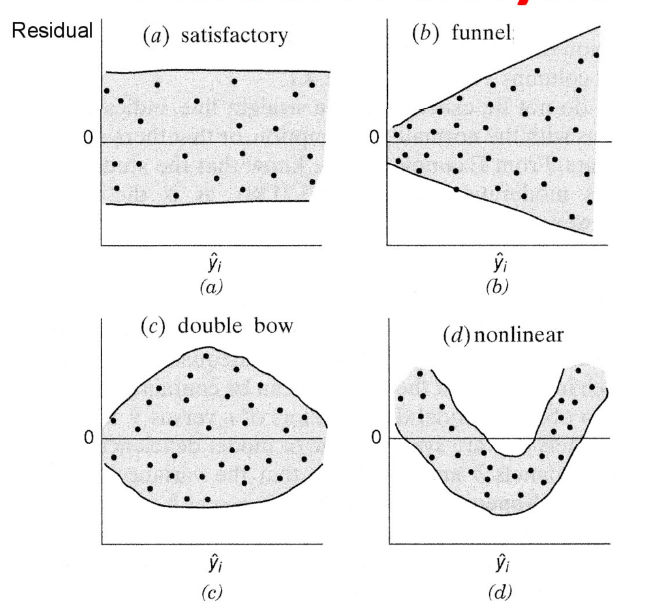
\includegraphics[width=0.45\textwidth]{1.png}
\end{figure}
However, the scale of residuals are largely dependent on the unit of the response. Therefore, we need to scaling them.
\begin{definition}[Standardized Residuals]
\normalfont Standardized residuals $d_i$ are defined from $e_i$ by
\[
d_i=\frac{e_i}{\sqrt{MS_\text{Res}}}
\]
\end{definition}
Here, the standardized residuals will have mean $0$ and \textit{approximately} unit variance. A large standardized residuals($d_j>3$) could potentially indicates outlier.\\
Since $\bm{e}=(\bm{I}-\bm{H})\bm{y}$, where $\bm{H}=\bm{X}(\bm{X}'\bm{X})^{-1}\bm{X}'$, by substituting $\bm{y}=\bm{X\beta}+\bm{\varepsilon}$, we will have
\[
\bm{e}=(\bm{I}=\bm{H})\varepsilon
\]
and covariance matrix of residuals
\[
\var(\bm{e})=\sigma^2(\bm{I}-\bm{H})
\]
\begin{definition}[Studentized Residuals]
\normalfont Studentized residuals is defined as
\[
\frac{e_i}{\sqrt{MS_\text{Res}}(1-h_{ii})}
\]
\end{definition}
\begin{definition}[PRESS Residual]
\normalfont PRESS Residual $e_{(i)}$ is defined as
\[
e_{(i)}=y_i-\hat{y}_{(i)}
\]
where $\hat{y_{(i)}}$ is the fitted value of the $i$th response based on all observations except the $i$th one.\\
We have
\[
e_{(i)}=\frac{e_i}{1-h_{ii}}
\]
The variance of $e_{(i)}$ is
\[
\var[e_{(i)}]=\frac{\sigma^2}{1-h_{ii}}
\]
Therefore, we can also define standardized PRESS Residual as
\[
\frac{e_{(i)}}{\sqrt{\var[e_{(i)}]}}=\frac{e_i}{\sqrt{\sigma^2(1-h_{ii})}}
\]
\end{definition}
\begin{definition}[R-Student]
\normalfont R-Student Residual $t_j$ is defined as
\[
t_i=\frac{e_i}{\sqrt{S^2_{(i)}(1-h_{ii})}}
\]
where $S^2_{(i)}$ is the estimat of $\sigma^2$ based on a data set with $i$th observation removed, i.e.
\[
S^2_{(i)}=\frac{(n-p)MS_\text{Res}-e_i^2/(1-h_{ii})}{n-p-1}
\]
\end{definition}
\subsection{Normal Probability Plot}
Suppose $X_1,\ldots, X_n\sim N(\mu, \sigma^2)$, let the CDF of $X_i$ be $F(x)$. Then, we have
\[
\frac{X_i-\mu}{\sigma}\sim N(0,1)
\]
and 
\[
F(\frac{X_i-\mu}{\sigma})\sim U(0,1)
\]
Suppose we order them in increasing order with $F(\frac{X_{(1)}-\mu}{\sigma})$ being the smallest, then
\[
F(\frac{X_{(i)}-\mu}{\sigma})\sim \text{Beta}(i, n+1-i)
\]
where
\[
E[F(\frac{X_{(i)}-\mu}{\sigma})]=\frac{i}{n+1}
\]
Therefore, heuristically we have
\[
F(\frac{X_{(i)}-\mu}{\sigma})\sim \frac{i}{n+1}
\]
in turn, we hrrive at
\[
\frac{X_{(i)}-\mu}{\sigma}\sim F^{-1}(\frac{i}{n+1})
\]
so
\[
X_{(i)}\sim \sigma F^{-1}(\frac{i}{n+1})+\mu
\]
Therefore, a \textbf{normal Q-Q} probability plot is obtained by plotting $X_{(i)}$ against $F^{-1}(\frac{i}{n+1})$.\\
A \textbf{normal P-P} probability plot is obtained by plotting $F(\frac{X_{(i)}-\mu}{\sigma})$ against $\frac{i}{n+1}$.
The plot is expected to be linear if the data set comes from a normal distribution.
\subsection{PRESS Statistic}
Recall that PRESS residuals $e_{(i)}=y_i-\hat{y}_{(i)}$, where $\hat{y}_{(i)}$ is the predicted value of the $i$th observed response based on a model fit to the remaining $n-1$ sample points.
\begin{definition}[PRESS Statistics]
\normalfont The PRESS statistics
\[
\text{PRESS}=\sum_{i=1}^n [y_i-\hat{y}_{(i)}]^2 = \sum_{i=1}^n (\frac{e_i}{1-h_{ii}})^2
\]
PRESS statistic can be used as measure of model quality, where a model with a small value of PRESS is desired.
\end{definition}
\subsection{Detection and Treatment of Outliers}
Residual plots against $\hat{y}_i$ and the normal probability plot are helpful in identifying outliers.
\subsection{Lack of Fit of Regression Model}
A lack of fit test requires replicated observations on the response $y$ for at least one level of $x$. These replicated observations are then used to obtain a \textbf{model independent estimate} of $\sigma^2$.\\
Suppose we have $n_i$ observations on the response at the $i$th level of the regressor $x_i$, where $i=1,\ldots, m$. Let $y_{ij}$ denote the $j$th observation on the response at $x_i$, where $j=1,\ldots, n_i$. There are $n=\sum_{i=1}^m n_i$ total observations.\\
We can decompose $SS_\text{Res}$ as 
\[
SS_\text{Res} = SS_\text{PE}+SS_\text{LOF}
\]
where $SS_\text{PE}$ is the sum of squares due to \textbf{pure error} and $SS_\text{LOF}$ is the sum of squares due to \textbf{lack of fit}.\\
In particular the above equation corresponds to the equation below
\[
\sum_{i=1}^m \sum_{j=1}^{n_i} (y_{ij}-\hat{y}_i)^2 = \sum_{i=1}^m \sum_{j=1}^{n_i}(y_{ij}-\bar{y}_i)^2+\sum_{i=1}^m n_i(\bar{y}_i-\hat{y}_i)^2
\]
Note, here $SS_\text{PE}$ is \textbf{model independent} estimate of $\sigma^2$.\\
Therefore, the test statistics is
\[
F_0=\frac{SS_\text{LOF}/(m-2)}{SS_\text{PE}/(n-m)}=\frac{MS_\text{LOF}}{MS_\text{PE}}
\]
where $E(MS_\text{LOF})=\sigma^2+\frac{\sum_{i=1}^m n_i[E(y_i)-\beta_0-\beta_1x_i]^2}{m-2}$, which will be close to $\sigma^2$ if there is no lack of fit.\\
We conclude that regression function is not linear if $F_0>F_{\alpha, m-2, n-m}$, and conclude there is no strong evidence of lack of fit otherwise. In the case of no lack of fit, both $MS_\text{PE}$ and $MS_\text{LOF}$ will be combined to estimate $\sigma^2$.
%\clearpage
\section{Transformation and Weighting to Correct Model Inadequacies}
In this section, we assume
\begin{enumerate}
  \item The model errors have mean zero and constant variance and are uncorrelated.
  \item The model errors have a normal distribution.
  \item The form of the model.
\end{enumerate}
The useful variable stabilizing transformations can be found in the table below:
\begin{table}[h]
\centering
\begin{tabular}{|c|c|}
\hline
Relationship of $\sigma^2$ to $E(y)$ & Transformation\\\hline
$\sigma^2\propto \text{constant}$ & $y'=y$\\\hline
$\sigma^2\propto E(y)$ & $y'=\sqrt{y}$\\\hline
$\sigma^2\propto E(y)[1-E(y)]$ & $y'=\sin^{-1}(\sqrt{y})$\\\hline
$\sigma^2\propto E(y)^2$ & $y'=\ln(y)$\\\hline
$\sigma^2\propto E(y)^3$ & $y'=y^{-\frac{1}{2}}$\\\hline
$\sigma^2\propto E(y)^4$ & $y'=y^{-1}$\\\hline
\end{tabular}
\end{table}
Sometimes, the model itself is not linear, therefore, we can linearise the model so that $y'=\beta_0+\beta_1x'$ for some transformed $y$ and $x$.
\subsection{Transformation on {$y$}: Box-Cox Method}
\begin{theorem}[Box Cox Method]
\normalfont We try to transform $\bm{y}=\bm{X\beta}+\bm{\epsilon}$ to $\bm{y}^{(\lambda)}=\bm{X\beta}+\bm{\epsilon}$ where
\[
y^{(\lambda)}=\begin{cases}
\frac{y^\lambda-1}{\lambda \bar{y}^{\lambda-1}}, & \lambda\neq 0\\
\bar{y}\ln y, & \lambda = 0\end{cases}
\]
where $\bar{y}=\frac{1}{\ln(\frac{1}{n}\sum_{i=1}^n\ln y_i)}$.
We select $\lambda$ to minimize the residual sum of squares from the regression of $y^\lambda$ on $x$.
\end{theorem}
Box-Cox Method transforms on $y$. We can also do transformation on $x$ such that $y=\beta_0+\beta_1x^\alpha+\epsilon$. To obtain the $\alpha$, we need to do the following iterations:
\begin{itemize}
  \item Let $\alpha_0 = 0$
  \item Denote $\xi=\begin{cases} x^\alpha, & \alpha \neq 0\\ \ln x, & \alpha = 0\end{cases}$.
  \item Taylor series $E(y)=f(\alpha)+(\alpha - \alpha_0)f'(\alpha_0) = \beta_0+\beta_1x+(\alpha-1)f'(\alpha_0)$
  \item Therefore, $E(y)=\beta_0+\beta_1x+\underbrace{(\alpha-1)\beta_1}_{\gamma}x^{\alpha_0}\ln x$.
  \item Use linear regression to find the estimators of above coefficients $\hat{\beta}_0$, $\hat{\beta}_1$ and $\hat{\gamma}$.
  \item Then we have $\alpha_1=\frac{\hat{\gamma}}{\hat{\beta}_1}+1$
\end{itemize}
\subsection{Generalized and Weighted Least Squares}
For \textbf{generalized least squares}, $\bm{y}=\bm{X\beta}+\bm{\epsilon}$, where $E(\bm{\epsilon})=0$ and $\var(\bm{\epsilon})=\sigma^2\bm{V}$, where this $V$ is non-singular and positive definite.\\
We have a non-singular symmetric matrix $\bm{K}$, where $\bm{KK}=\bm{V}$.\\
Define $\bm{z}=\bm{K}^{-1}\bm{y}$, $\bm{B}=\bm{K}^{-1}\bm{X}$ and $\bm{g}=\bm{K}^{-1}\bm{\epsilon}$. This gives
\[
\bm{z}=\bm{B\beta}+\bm{g}
\]
with $E(\bm{g})=\bm{0}$ and $\var{\bm{g}}=\sigma^2\bm{I}$.\\
Therefore, $S(\bm{\beta})=(\bm{y}-\bm{X\beta})'\bm{V}^{-1}(\bm{y}-\bm{X\beta})$, and least square normal equation is $(\bm{X}'\bm{V}^{-1}\bm{X})\hat{\bm{\beta}}=\bm{X}'\bm{V}^{-1}\bm{y}$, so
\[
\hat{\bm{\beta}}=(\bm{X}'\bm{V}^{-1}\bm{X})^{-1}\bm{X}'\bm{V}^{-1}\bm{y}
\]
and $\hat{\bm{\beta}}$ is an unbiased estimator of $\bm{\beta}$.\\
We have $\var{\hat{\bm{\beta}}}=\sigma^2(\bm{B}'\bm{B})^{-1}=\sigma^2(\bm{X}'\bm{V}^{-1}\bm{X})^{-1}$.\\
The ANOVA table is as followed
\begin{figure}[h]
\centering
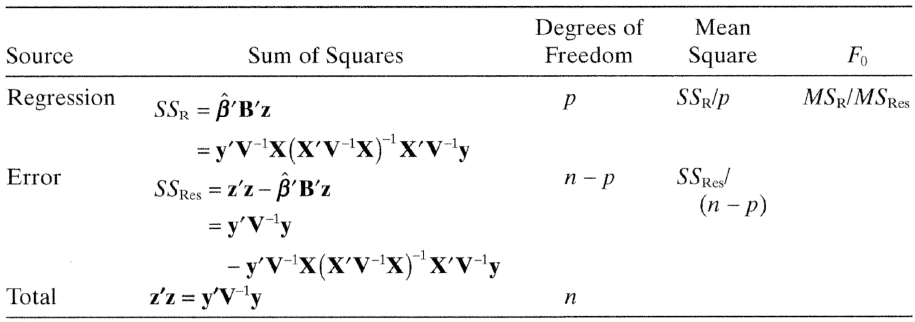
\includegraphics[width=0.45\textwidth]{2.png}
\end{figure}
\begin{theorem}[Weighted Least Square]
\normalfont Weighted Least Square is the special case of generalized least square where
\[
\sigma^2 \bm{V}=\sigma^2\begin{pmatrix}\frac{1}{w_1}&&0\\&\ddots&\\0&&\frac{1}{w_n}\end{pmatrix}
\]
So $\bm{W}=\bm{V}^{-1}$. Therefore, \[
\hat{\bm{\beta}}=(\bm{X}'\bm{W}\bm{X})^{-1}\bm{X}'\bm{W}\bm{y}
\]
The transformed matrix $\bm{B}=\begin{pmatrix}1\sqrt{w_1} & x_{11}\sqrt{w_1}\cdots x_{1k}\sqrt{w_1}\\1\sqrt{w_2} & x_{21}\sqrt{w_2}\cdots x_{2k}\sqrt{w_2}\\\cdots&\cdots& \ddots&\cdots\\1\sqrt{w_n} & x_{n1}\sqrt{w_n}\cdots x_{nk}\sqrt{w_n}\end{pmatrix}$ and $\bm{Z}=\begin{pmatrix}y_1\sqrt{w_1}\\y_2\sqrt{w_2}\\\vdots\\y_n\sqrt{w_n}\end{pmatrix}$.
\end{theorem}
%\clearpage
\section{Diagonistics for Leverage and Influence}
\begin{definition}
\normalfont Leverage is a measure of the effect of an observation $i$ on the predicted value.\\
The \textbf{leverage} of the observation $i$ is $h_{ii}$ where $h_{ii}=\bm{x}_i'(\bm{X}'\bm{X})^{-1}\bm{x}_i$ where $\bm{x}_i'$ is the $i$th row of the $\bm{X}$ matrix.\\
Also, we note that $\bar{h}=\frac{1}{n}\sum_{i=1}^n h_{ii}=\frac{p}{n}$.\\
Any observation $i$ for which $h_{ii}$ exceeds $2\bar{h}=2\frac{p}{n}$ is remote enough from the rest of the data and is considered a \textbf{leverage point}.
\end{definition}
\textbf{Remark}: Not all leverage points are going to be influential on regression coefficients. Usually, a point is influential if it deteriorates $MS_\text{Res}$ a lot.\\
More precisely, we use Cook's Distance as a measure of \textbf{influence}.
\begin{definition}[Cook's Distance]
\normalfont Let $\hat{\bm{\beta}}$ be the estimate based on all $n$ points and $\hat{\bm{\beta}}_{(i)}$ be the estimate obtained by deleting the $i$th point. Then the Cook's distance for the $i$th point is defined to be
\[
D_i=\frac{(\hat{\bm{\beta}}_{(i)}-\hat{\bm{\beta}})'\bm{X}'\bm{X}(\hat{\bm{\beta}}_{(i)}-\hat{\bm{\beta}})}{pMS_\text{Res}}
\]
Points with large values of $D$ have considerable influence on the least-square estimates $\hat{\bm{\beta}}$.\\
The magnitude of $D_i$ is usually assessed by comparing it to $F_{\alpha, p, n-p}$ and since $F_{0.5, p, n-p}\approx 1$, we usually consider points for which $D_i>1$ to be influential.
\end{definition}
Cook's distance can be calculated via alternative formula: 
\[
D_i=\frac{r_i^2}{p}\frac{\var(\hat{y}_i)}{\var(e_i)}=\frac{r_i^2}{p}\frac{h_{ii}}{1-h_{ii}}
\]
where $r_i$ is the $i$th studentized residual.\\
Also, we can write $D_i$ as
\[
D_i=\frac{(\hat{\bm{y}}_{(i)}-\hat{\bm{y}})'(\hat{\bm{y}}_{(i)}-\hat{\bm{y}})}{pMS_\text{Res}}
\]
Measure of influence can also include DFFITS and DFBETAS.
\begin{definition}[DFBETAS]
\normalfont We define $DFBETAS_{j,i}$ on the $j$th regression coefficient with respect to $i$th observation.
\[
DFBETAS_{j,i}=\frac{\hat{\beta}_j-\hat{\beta}_{j(i)}}{\sqrt{S_{(i)}^2C_{jj}}}
\]
where $C_{jj}$ is the $j$th diagonal elements of $(\bm{X}'\bm{X})^{-1}$, $S_{(i)}^2$ is the estimate of $\sigma^2$ based on a data set with $i$th observation removed, and $\hat{\beta}_{j(i)}$ is the $j$th regression coefficient computed without use of $i$th observation.\\
A large value of $DFBETAS_{j,i}$ indicates that observation $i$ has considerable influence on the $j$th regression coefficients.\\
\end{definition}
Similarly, we define $DFFITS_i$.
\begin{definition}[DFFITS]
\normalfont We define $DFFITS_i$ on the $i$th predicted $y_i$.
\[
DFFITS_i=\frac{\hat{y}_i-\hat{y}_{(i)}}{\sqrt{S_{(i)}^2h_{ii}}}
\]
where $\hat{y}_{(i)}$ is the fitted value of $y_i$ obtained without the use of $i$th observation.\\
$DFFITS_i$ is the number of standard deviations that the fitted value $\hat{y}_i$ \textbf{changes} if observation $i$ is removed. (Note: $\var(\hat{y}_i))=\sigma^2h_{ii}$)
\end{definition}
An alternative formula for $DFFITS_i$ is 
\[
DFFITS_i=\frac{h_{ii}}{1-h_{ii}}^{\frac{1}{2}}t_i
\]
where $t_i$ is the R-student residual.\\
Therefore, if the data point is an outlier, then R-student will be large in magnitude while if data has high leverage, $h_{ii}$ will be close to unity. In either case $DFFITS_i$ is large.\\
The cutoff value suggested for $DFFBETAS_{j,i}$ and $DFFITS_i$ is
\begin{itemize}
  \item $|DFBETAS_{j,i}|>\frac{2}{\sqrt{n}}$ 
  \item $|DFFITS_i|>2\sqrt{\frac{p}{n}}$
\end{itemize}
\subsection{A Measure of Model Performance}
\begin{definition}[Generalised Variance]
\normalfont The overall precision of estimation can be measured using \textbf{generalized variance} $GV$:
\[
GV(\hat{\bm{\beta}})=|\var(\hat{\bm{\beta}})|=|\sigma^2(\bm{X}'\bm{X})^{-1}|
\]
To express the role of $i$th observation on the preision of estimation, define $COVRATIO_i$ to be
\[
COVRATIO_i=\frac{|(\bm{X}_{(i)}'\bm{X}_{(i)})^{-1}S_{(i)}^2|}{(\bm{X}'\bm{X})^{-1}MS_\text{Res}}
\]
If $COVRATIO_i>1$, the $i$th observation improves the precision of estimation, whereas a less than 1 $COVRATIO_i$ suggesta that inclusion of $i$th point degrades precision.
\end{definition}
The suggested cutoff values for $COVRATIO_i$: if $COVRATIO_i>1+\frac{3p}{n}$ or if $COVRATIO_i<1-\frac{3p}{n}$, ten the $i$th point should be considered influential. The lower bound is appropriate if $n>3p$. These cutoffs are only recommended for large samples.
%\clearpage
\section{Polynomial Regression Models}
\subsection{Polynomial Models}
$k$th order polynomial model in one variable is in the form of
\[
y=\beta_0+\beta_1x+\beta_2x^2+\cdots+\beta^kx^k+\varepsilon
\]
The definition can extend to $k$th order polynomial model in many variables. For example, the second-order polynomial in 2 variables is in the form of
\[
y=\beta_0+\beta_1x_1+\beta_2x_2+\beta_{11}x_1^2+\beta_{22}x_2^2+\beta_{12}x_1x_2+\varepsilon
\]
There are a few important considerations when fitting a polynomial in one variable:
\begin{enumerate}
  \item \textbf{Order of the model} should be kept as \textbf{low} as possible.
  \item \textbf{Model-Building Strategy}: forward selection or backward elimination.
  \item \textbf{Extrapolation} should be avoided
  \item \textbf{Ill-COnditioning I}. As order of polynomial increases, the $\bm{X}'\bm{X}$ matrix becomes ill-conditioned.\\\textbf{Solution}: Non-essential ill-conditioning caused by arbitrary choice of origin can be removed by first centering the regressor variables, i.e. $x\to x-\bar{x}$.
  \item \textbf{Ill-Conditioning II}. If values of $x$ are limited to a narrow range, there can be significant ill-conditioning and multicollinearity in the columns of $\bm{X}$ matrix.
  \item \textbf{Hierarchy}. A model is \textbf{hierarchical} if the power of varaible is continuous.\\Only hierarchical models are invariant under linear transformation of $x$, which means both models will produce the same predicted values, residuals, $R^2$, etc.
\end{enumerate}
\subsection{Piecewise Polynomial Fitting(Splines)}
Splines are piecewise polynomial of order $k$. The joint points of the pieces are called \textbf{knots}.
\begin{definition}[Cubic Spline]
\normalfont A cubic spline with $h$ knots, $t_1<\cdots<t_h$ with continuous first and second derivatives can be written as
\[
S(x)=\sum_{j=0}^3\beta_{0j}x^j+\sum_{i=1}^h\beta_i(x-t_i)_{+}^3
\]
where
\[
(x-t_i)_{+}=\begin{cases}
(x-t_i)&\text{ if }x-t_i>0\\
0&\text{ if }x-t_i\leq 0
\end{cases}
\]
\end{definition}
Generally, we require function values and $k-1$ derivatives to agree on the knots, so that the spline is a continous functin with $k-1$ continuous derivatives. To do this, we need to assume the position of the knots are known.\\
\begin{definition}[Cubic Spline with No Continuity Restriction]
\normalfont 
\[
S(x)=\sum_{j=0}^3 \beta_{0j}x^j+\sum_{i=1}^h\sum_{k=0}^3\beta_{ij}(x-t_i)_{+}^j
\]
\end{definition}
\begin{theorem}[Hypothesis Testing of Cubic Spline]
\normalfont 
\begin{itemize}
  \item $H_0:\beta_0=0$ tests continuity of $S(x)$.
  \item $H_0:\beta_0=\beta_1=0$ tests continuity of $S(x)$ and $S'(x)$.
  \item $H_0:\beta_0=\beta_1=\beta_2=0$ tests continuity of $S(x)$, $S'(x)$ and $S''(x)$.
  \item $H_0:\beta_0=\beta_1=\beta_2=\beta_3=0$ tests single cubic polynomial fits data better than a cubic spline over range of $x$.
\end{itemize}
\end{theorem}
Cubic Spline model is good as fitting it can be treated as fitting a mutiple linear regression model.\\
In general, we can have linear spline just by changing the formula's power, for both the continuous and discontinuous case.
\subsection{Non-parametric Regression}
In paramatric model, we have a proposed equation and we try to find the corresponding unknown coefficient(s). In Non-parametric model, we do not have a proposed equation.
\begin{definition}[Kernel Regression]
\normalfont We estimate the $i$th response in this way (called kernel smoother estimation)
\[
\tilde{y}_i=\sum_{j=1}^n w_{ij}y_j
\] 
where 
\[
w_{ij}=\frac{K(\frac{x_{i}-x_{j}}{b})}{\sum_{k=1}^n K(\frac{x_{i}-x_{k}}{b})}
\]
and $K(t)=\begin{cases} 1, &|t|\leq 0.5\\0, & |t|>0.5\end{cases}$.\\
Essentially, $K$ will be $0$ if and only if for that particular $i$ and $J$, $x_i-x_j\leq \frac{b}{2}$. This is known as Box kernel.
\end{definition}
The properties of kernel smoother depend much more on choice of bandwidth $b$ than actual kernerl function. Other kernel functions can be found in lecture notes.
\subsection{Locally Weighted Regression(LOESS)}
Let $x_0$ be specific location of interest. We pick a span $d$, and let the $\delta(x_0)$ be the distance of the farthest point in the neighbourhood $[x_0-d,x_0+d]$. For another point $x_j$, the weight is $W(\frac{|x_0-x_j}{\delta(x_0)})$ where $W(t)=\begin{cases} (1-t^3)^3 &\text{ for }0\leq <1\\0&\text{ elsewhere}\end{cases}$.
We then use all points in the neighbourhood to generate a \textbf{weighted least-squares estimate} of the specific response $x_0$.
\subsection{Estimating {$\sigma^2$}}
Here estimator $\tilde{\bm{y}}=\bm{Sy}$ is a linear function in $\bm{y}$, regardless whether our model is parametric or not. For example, in multiple linear regression, we have $\hat{\bm{y}}=\bm{Hy}$.\\
Therefore, we have 
\[
SS_\text{Res}=(\bm{y}-\bm{Sy})'(\bm{y}-\bm{Sy})=\bm{y}'[\bm{I}-\bm{S}'-\bm{S}+\bm{S}'\bm{S}]\bm{y}
\]
And
\[
E(SS_\text{Res})=\tr[(\bm{I}-\bm{S}'-\bm{S}+\bm{S}'\bm{S})\bm{\sigma}^2\bm{I}]=\sigma^2[n-2\tr(\bm{S})+\tr(\bm{S}'\bm{S})]
\]
Therefore, an estimator of $\bm{\sigma}^2$ is
\[
\tilde{\sigma}^2=\frac{\sum_{i=1}(y_i-\tilde{y}_i)^2}{n-2\tr(\bm{S})+\tr(\bm{S}'\bm{S})}
\]
and also
\[
R^2=\frac{SS_\text{T}-SS_\text{Res}}{SS_\text{T}}
\]
\subsection{Polynomial Models in Two or More Variables}
An example of a two-variable quadratic model is $y=\beta_0+\beta_1x_1+\beta_2x_2+\beta_{11}x_1^2+\beta_{22}x_2^2+\beta_{12}x_1x_2+\epsilon$.\\
We can use repeated experiment to get an independent estimate of $\sigma^2$ so as to test lack of fit.\\
We can transform the regressor variable to an indicator variable. This reduces the complexity of $\bm{X}$ matrix.\\
To fit a quadratic model, we usually requires four points in a rectangular fashion. We can add some more experiments in the cross manner.
\subsection{Rotability}
$\sqrt{\var[\hat{y}(\bm{x}_0)]}$ is the same for all points $\bm{x}_0$ that are the same distance from the center of the design. This is desirable, and this is how we introduce the points in experiment.
\subsection{Orthogonal Polynomials}
Suppose the model $y_i=\beta_0+\beta_1x_i+\beta_2x_i^2+\cdots+\beta_kx_i^k+\epsilon_i$. Generally, the column of $\bm{X}$ matrix will not be orthogonal.\\
Now suppose that we fit the model
\[
y_i=\alpha_0P_0(x_i)+\alpha_1P_1(x_i)+\cdots +\alpha_kP_k(x_i)+\epsilon
\]
where $P_u(x_i)$ is a $u$th order orthogonal polynomial defined such that
\[
\sum_{i=1}^n P_r(x_i)P_s(x_i)=0, r\neq s\forall r,s=0,\ldots, k
\]
and $P_0(x_i)=1$.\\
Then the model becomes $\bm{y}=\bm{X\alpha}+\bm{\epsilon}$, where $\bm{X}=\begin{pmatrix}P_0(x_1)\cdots P_k(x_1)\\\vdots &\ddots&\vdots\\P_0(x_n)&\cdots&P_k(x_n)\end{pmatrix}$.\\
Due to orthogonality, we have the nice property:
\[
\bm{X}'\bm{X}=\text{diag}[\sum_{i=1}^n P_0^2(x_i), \ldots, \sum_{i=1}^n P_k^2(x_i)]
\]
The least square estimators of $\alpha$ are found from $(\bm{X}'\bm{X})^{-1}\bm{X}'\bm{y}$:
\[
\hat{\alpha}_j=\frac{\sum_{i=1}^n P_j(x_i)y_i}{\sum_{i=1}^n P_j^2(x_i)}
\]
Since, we set $P_0(x_i)=1$, we have $\hat{\alpha}_0=\bar{y}$.\\
The residual sum of squares is
\[
SS_\text{Res}(k)=SS_\text{T}-\sum_{j=1}^k\hat{\alpha}_j[\sum_{i=1}^n P_j(x_i)y_i]
\]
The regression sum of sequares for any model parameter does not depend on the other parameters in teh model. The regression sum of squares is
\[
SS_\text{R}(\alpha_j):=SS_\text{R}(\alpha_j\mid \alpha_0,\cdots, \alpha_{j-1},\alpha_{j+1},\cdots,\alpha_k)=\hat{\alpha}_j\sum_{i=1}^nP_j(x_i)y_i:=SS_\text{R}(\alpha_j\mid \alpha_0)
\]
The last equality comes from orthogonality.\\
To test $H_0=\alpha_k=0$, we need 
\[
F_0=\frac{SS_\text{R}(\alpha_k)}{SS_\text{Res}(k)/(n-k-1)}
\]
The orthogonal polynomials $P_j(x_i)$ can be easily constructed if the levels of $x$ are equally spaced. For explicit formula, look into lecture notes.
%\clearpage
\section{Indicator Variables}
There are two types of variables: quantitative variables and qualitative/categorical variables.\\
A qualitative variable has no natural scale of measurement. \\
We can use indicator variables to indicate whether a variable should be considered in the model.\\
We can use the indicator variable in or not in interaction terms.\\
If there is no interaction, we only need to test the coefficient of indicator.\\
If there is interaction term, we also need to test for interaction term.
\subsection{Special Case Testing}
We are interested in testing 3 cases, namely parallel lines, concurrent lines and coincident lines.
\subsubsection{Parallel Lines}
Two lines are parallel if their slopes are equal and we allow the $y$-intercepts to differ.\\
For example, for the model $y=\beta_0+\beta_1x_1+\beta_2x_2+\beta_{12}x_1x_2+\epsilon$, $x_2\in\{0,1\}$ is an indicator variable that allows both slope and $y$ intercept to differ. 
\begin{itemize}
  \item Suppose $x_2=0$, we have $y=\beta_0+\beta_1x_1+\epsilon$
  \item Suppose $x_2=1$, we have $y=(\beta_0+\beta_2)+(\beta_1+\beta_{12})x_1+\epsilon$
\end{itemize}
To test for parallel lines, we test $H_0:\beta_{12}=0$.\\
For multiple indicator variables $x_2,\ldots, x_n$, the genral model with interaction terms is
\[
y=\beta_0+\beta_1x_1+\sum_{i=2}^n (\beta_ix_i+\beta_{1i}x_1x_i)+\epsilon
\]
and we test $H_0=\beta_2=\cdots=\beta_n=0$
\subsubsection{Concurrent Lines}
Concurrent lines are lines where their $y$-intercepts are the same and we allow the slopes to differ.\\
Using the model above, we are testing $H_0:\beta_2=\cdots=\beta_n=0$.
\subsubsection{Coincident Lines}
Coincident lines are lines where they have the same slope as well as the same $y$-intercept.\\
Using the model above, we are testing $H_0:\beta_2=\cdots=\beta_n=0$, and $\beta_{12}=\cdots=\beta_{1n}=0$.
\subsection{Indicator Variable versus Regression on Allocated Codes}
The difference between indicator variable against allocated codes is that
\begin{itemize}
  \item Each indicator variable is only binary, i.e., $\{0,1\}$, one level is represented by a $1$ for that particular variable and $0$ for anything else, and each variable will become a regressor variable.
  \item Allocated codes is just different assignement of values in \textbf{one} variable to represent different levels, and turns to only one regressor variable.
\end{itemize}
However, allocated codes do not work well. This is because, $E(y\mid x_1,x_{i+1})-E(y\mid x_1,x_i)=\beta$ for all $i$, which doesn't make sense, as it imposes a particular metric on the levels of the qualitative factor.
\subsection{Indicator Variable as a Substitute for a Quantitative Regressor}
We can represent a range of quantitative variable as a set of indicator variables. However, it has the disadvantage that more parameters are required to represent the information content.\\
However, an advantage of the indicator variable approach is that it \textit{does not} require the analyst to make any prior assumptions about the \textbf{functional form of the relationship} between the response and the regressor variable.
\subsection{Pooled Two-sample {$t$} Procedure}
Suppose that an Simple Random Sample of size $n_1$ is drawn from a Normal population with unknown mean $\mu_1$ and that an independent SRS of size $n_2$ is drawn from another Normal population with unknown mean $\mu_2$. Suppose also that the two population have the \textbf{same standard deviation}.\\
To test the hypothesis that $H_0:\mu_1=\mu_2$ against alternative $H_1:\mu_1\neq \mu_2$, we use test statistic
\[
t=\frac{\bar{x}_1-\bar{x}_2}{s_p\sqrt{\frac{1}{n_1}+\frac{1}{n_2}}}
\]
where $s_p^2$ is the pooled estimators of $\sigma^2$, in the form of
\[
s_p^2=\frac{(n_1-1)s_1^2+(n_2-1)s_2^2}{n_1+n_2-2}
\]
Here, we can treat the two variables coming from two binary choices of the same categorical variable.\\
One way ANOVA is a generalization of the pooled two-sample $t$ procedure. \\
In one-way ANOVA, let $k$ denote number of levels and $n$ denote number of observations per level.\\
For the model for one-way classification analysis of variance we have
\[
y_{ij}=\mu+\tau_i+\epsilon_{ij}, \text{ where }i=1,\ldots, k,\;\;\;\;j=1,\ldots, n
\]
and the regression model is
\[
y_{ij}=\beta_0+\sum_{p=1}^{k-1}\beta_px_{pj}+\epsilon_{ij}, \text{ where }i=1,\ldots, k,\;\;\;j=1,\ldots, n
\]
Here, $x_1,\ldots, x_{k-1}$ are $k-1$ indicator variables, used to represent $k$ levels.\\
The connection between the two models is that they share the same ANOVA table.\\
For the experimental design model, $\mu$ is the common mean, $\tau_i$ is the binary variable, which equals $1$ if it comes from the $i$th level and $0$ otherwise.\\
For the regression model, we can create a matrix $X:=\mathbb{R}^{kn\times (1+k)}$ where $M=(1, 1_{\tau_1},\ldots, 1_{\tau_k})$. However, the matrix is firstly, not linearly independently on a column basis, which makes $X'X$ singular. Therefore, we impose an additional constraint:
\[
\sum_{i=1}^k\tau_i = 0\;\;\;(\ast)
\]
And the matrix $X=(1, 1_{\tau_1}-1_{\tau_k}, \cdots, 1_{\tau_{k_1}}-1_{\tau_k)}$.\;\

After we get this $X$, we can solve the actual value $\mu$ and $\tau$ by solving
\[
(X'X)\begin{pmatrix} \mu\\\tau_1\\\vdots\\\tau_k\end{pmatrix}=X'y
\]
The ANOVA table obtained will be
\begin{table}[h]
\centering
\begin{tabular}{|c|c|c|c|c|}
\hline
 & Sum. Sqs & DF & Mn Sq & $F_0$\\\hline
Treat & $\displaystyle n\sum_{i=1}^k(\bar{y}_{i\cdot}-\bar{y}_{\cdot\cdot})^2$ & $k-1$ & $\frac{SS_\text{Treat}}{k-1}$ & $\displaystyle\frac{MS_\text{Treat}}{MS_\text{Res}}$\\\hline
Error & $\displaystyle\sum_{i=1}^k\sum_{j=1}^n (y_{ij}-\bar{y}_{i\cdot})^2$ & $k(n-1)$ & $\frac{SS_\text{Res}}{k(n-1)}$ & \\\hline
Total & $\displaystyle\sum_{i=1}^k\sum_{j=1}^n (y_{ij}-\bar{y}_{\cdot\cdot})^2$ & $kn-1$ & & \\\hline
\end{tabular}
\end{table}
We can use the regression model too, where we arrive at the same regressor and ANOVA.\\
We can use the ANOVA table's $F_0$ to test
\[
H_0:\tau_1=\cdots=\tau_k=0\text{ against } H_1:\tau_i\neq 0\text{ for at least one }i
\]
The relationship between parameters of regression model and paramaters of Analysis of Variance model is that
\[
\beta_0=\mu_k, \beta_i=\mu_i-\mu_k, i = 1,\ldots, k-1
\]
%\clearpage
\section{Multicollinearity}
If there is no linear relationship between regressors, they are said to be \textbf{orthogonal}. When there are \textbf{near-linear} dependencies among the regressors, the problem of \textbf{multicollinearity} is said to exist.
To observe multicollinearity, we need to use unit-length scaling on $X$: $y\to \frac{y-\mu_y}{\sigma_y\sqrt{n-1}}$. We then compute the correlation coefficients via $\bm{X}'\bm{X}$.
\begin{theorem}[Eigenvalue Decomposition]
\normalfont We can decompose $A$ to be $A=T\Lambda T'$ where $T=(t_1,\ldots, t_p)$ are $p$ orthogonal eigenvectors of $A$, and $\Lambda = \text{diag}[\lambda_1,\ldots, \lambda_p]$ where $\lambda_1,\ldots, \lambda_p$ are $p$ \textit{positive} eignevalues of $A$.\\
With this setup, we have 
\begin{itemize}
  \item $\tr(A)=\sum_{i=1}^p \lambda_i$
  \item $\tr(A')=\sum_{i=1}^p 1/\lambda_i$.
\end{itemize}
\end{theorem}
\subsection{Source of Multicollinearity}
Given the multiple regression model $\bm{y}=\bm{X\beta}+\bm{\epsilon}$, if we have scaled the regressor variables and response to unit length, then $\bm{X}'\bm{X}$ is a matrix of correlations between regressors, whereas $\bm{X}'\bm{y}$ is a vector of correlation between regressors and the response.\\
Let $j$th column of $\bm{X}$ matrix be $\bm{X}_j$. Then we say $X_1,\ldots, X_p$ will be linearly dependent if there is a set of constants $t_1,\ldots, t_p$ not all zero, such that $\sum_{j=1}^p t_j\bm{X}_j=\bm{0}$.\\
The sum above is a vector of constant $\bm{m}$ if regressor are not centered.\\
If the above equation holds exactly for a subset of columns of $\bm{X}$, then the rank of $\bm{X}'\bm{X}$ matrix is less than $p$ and inverse does not exist. \\
If above equation is approximately true for some subsets of columns of $\bm{X}$, then tehre will be a near-linear dependency in $\bm{X}'\bm{X}$ and problem of multicollinearity is said to exist.\\
Therefore, we can see multicolinerality as a form of ill-conditioning in the $\bm{X}'\bm{X}$ matrix. \\
There are four primary sources of multicollinearity:
\begin{enumerate}
  \item The data collection method employed, where the data is only sampled from a subspace of region of regressors.
  \item Constraints on the model or in the population
  \item Model Specification, whether we center the data
  \item An overdefined model, which has more regressor variables than observations.
\end{enumerate}
\subsection{Effect of Multicollinearity}
Suppose there are only two regressor variable $x_1,x_2$ and model
\[
y=\beta_1x_1+\beta_2x_2
\]
have $x_1,x_2,y$ scaled to unit length. We have, for $(\bm{X}'\bm{X})\hat{\bm{\beta}}=\bm{X}'\bm{y}$,
\[
\begin{pmatrix}1 & r_{12}\\ r_{12} & 1\end{pmatrix}\begin{pmatrix}\hat{\beta_1}\\\hat{\beta}_2\end{pmatrix} = \begin{pmatrix} r_{1y}\\r_{2y}\end{pmatrix}
\]
where $r_{12}$ is the simple correlation between $x_1$ and $x_2$, and $r_{iy}$ is the simple correlation between $x_i$ and $y$.\\
Then we have
\[
\bm{C}:=(\bm{X}'\bm{X})^{-1}=\begin{pmatrix} \frac{1}{1-r_{12}^2} & \frac{-r_{12}}{1-r_{12}^2}\\ \frac{-r_{12}}{1-r_{12}^2} & \frac{1}{1-r_{12}^2}\end{pmatrix} 
\]
and $\hat{\beta}_1 = \frac{r_{1y}-r_{12}r_{2y}}{1-r_{12}^2}$, $\hat{\beta}_2 = \frac{r_{2y}-r_{12}r_{1y}}{1-r_{12}^2}$.
Strong multicolliearity between $x_1$ and $x_2$ will cause $r_{12}$ to be large. This results, the variance of $\hat{\beta}_j$ and $\cov(\hat{\beta}_1,\hat{\beta}_2)$ is very large.\\

When there are more than two regressor variables, diagonal elements of $\mathbf{C}$ has $C_{jj}=\frac{1}{1-R_j^2}$ and $\var(\hat{\beta}_j)=C_{jj}\sigma^2$.\\
Where $R_j^2$ is the coefficient of multiple determination from the regression of $x_j$ on the remaining $p-1$ regressors. \\
If there is strong multicollinearity between $x_i$ and any subset of the other $p-1$ regressors, then the value of $R_i^2$ will be close to unity.\\
Generaly, the covariance between two $\beta$ will also be large if the corresponding regressor are involved in a multicollinear relationship.\\
Multicollinearity also tends to produce least-square estimates $\hat{\beta}_j$ that are twoo large in absolute value.\\
The square distance $L_1^2$ is defined as 
\[
L_1^2=(\hat{\bm{\beta}}-\bm{\beta})'(\hat{\bm{\beta}}-\bm{\beta})
\]
The expected squared distance $E(L_1^2)=\sigma^2\tr(\bm{X}'\bm{X})^{-1}$.\\
Here, $E(L_1^2)=\sigma^2\sum_{j=1}^p \frac{1}{\lambda_j}$. When the multicollinearity present, some of the eigenvalues of $\bm{X}'\bm{X}$ will be small, which makes this expectation large. So we just need to check eigenvalues.\\
We have
\[
E(\hat{\bm{\beta}'\bm{\beta}}) = \bm{\beta}'\bm{\beta} + \sigma^2\tr(\bm{X}'\bm{X})
\] 
\subsection{Multicollinearity Diagonostics}
Techniques for detecting multicollinearity include
\begin{itemize}
  \item Examination of Correlation Matrix, which detects only correlation between 2 variables.
  \item Variance Inflation Factors
  \item Eigensystem Analysis of $\bm{X}'\bm{X}$
\end{itemize}
\subsubsection{Variance Inflation Factors}
We look at matrix $\mathbf{C}:=(\bm{X}'\bm{X})^{-1}$, which gives the $\var{\hat{\beta}}:=\sigma^2\mathbf{C}$. The variance inflation factor is defined by diagonal element of this matrix. If the regressor variable is \textbf{centered}, we have 
\[
VIF_j=C_{jj}=(1-R_j^2)^{-1}
\]
If $x_j$ is nearly orthogonal to remaining regressors, $R_j^2$ is small and $C_jj$ is close to unity. However, if $x_j$ is nearly dependent on some subset of remaining regressors, $R_j^2$ is nearly unity and $C_jj$ is large. We can view $C_{jj}$ as the factor by which the variance of $\hat{\beta}_1$ is increased due to near-linear dependencies among the regressors.
\subsubsection{Eigensystem analysis of {$\bm{X}'\bm{X}$}}
The characteristic roots, or \textbf{eigenvalues} of $\bm{X}'\bm{X}$, say $\lambda_1,\ldots, \lambda_p$, can be used to measure the extent of multicollinearity in the data.\\
If there are one or more near-linear dependencies in the data, then one or more of the eignevalues will be small. One or more small eignevalues imply that there are near-linear dependencies among the $\bm{X}$.\\
Specifically, we compute the \textbf{condition number} of $\bm{X}'\bm{X}$
\[
\kappa = \frac{\lambda_{\max}}{\lambda_{\min}}
\]
If the condition number is less than $100$, there is no serious problems with multicollinearity. Condition numbers betwween 100 and 1000 implies moderate to strong multicollinearity and if $\kappa$ exceeds $1000$, severe multicollinearity is indicated.\\
The \textbf{condition incides} of the $\bm{X}'\bm{X}$ matrix are 
\[
\kappa_j=\frac{\lambda_{\max}}{\lambda_j},\;\;\;j=1,\ldots, p
\]
\subsubsection{Singular-Value Decomposition}
The $n\times p$ $\bm{X}$ matrix may be decomposed as
\[
\bm{X}=\bm{UDT}'
\]
where $\bm{U}$ is $n\times p$, $\bm{U}'\bm{U}=\bm{I}$. $\bm{T}$ is $p\times p$, where $\bm{T}$ is the matrix of eigenvectors of $\bm{X}'\bm{X}$, and $\bm{T}'\bm{T}=\bm{I}$, and $\bm{D}$ is a $p\times p$ diagonal matrix with nonnegative diagonal elements $\mu_j$. The $\mu_j$'s are called \textbf{singular values} of $\bm{X}$.\\
Note, the squares of singular values of $\bm{X}$ are the eigenvalues of $\bm{X}'\bm{X}$.
\subsection{Methods for Dealing with Multicollinearity}
We can deal with multicollinearity by
\begin{itemize}
  \item Collecting additional data
  \item Model Respecification(centering)
  \item Ridge regression
  \item Pricipal component regression
\end{itemize}
\subsubsection{Ridge Regression}
To understand ridge regression, we need to understand mean squared error. Suppose $\hat{\theta}$ is an estimator of $\theta$, then
\begin{itemize}
  \item $\bar(\hat{\theta}-\theta)=E[(\hat{\theta}-\theta)^2]-[E(\hat{\theta}-\theta)]^2$.
  \item $\var{\hat{\theta}}=E[(\hat{\theta}-\theta)^2]-[E(\hat{\theta})-\theta]^2$.
  \item $MSE(\hat{\theta})=E[(\hat{\theta}-\theta)^2]=\var(\hat{\theta})+[E(\hat{\theta})-\theta]^2$
  \item If $E(\hat{\theta})=\theta$, $MSE(\hat{\theta})=\var(\hat{\theta})$
\end{itemize}
Suppose a vector $\hat{\bm{\theta}}$ is an estiamtor of $\bm{\theta}$, then
\begin{align*}
MSE(\hat{\bm{\theta}})&=\tr(E[(\hat{\bm{\beta}}-\bm{\beta})(\hat{\bm{\beta}}-\bm{\beta})'])\\
&=E[(\hat{\bm{\beta}}-\bm{\beta})(\hat{\bm{\beta}}-\bm{\beta})']\\
&=\sum_{i=1}^p E[(\hat{\beta}_i-\beta_i)^2]\\
&=\sum_{i=1}^p (\var(\hat{\beta}_i-\beta_i)+[E(\hat{\beta}_i-\beta_i)]^2)\\
&=\sum_{i=1}^p \var(\hat{\beta}_i)+\sum_{i=1}^p [E(\hat{\beta}_i)-\beta_i]^2
\end{align*}
The problem with method of least squares is the requirement that $\hat{\bm{\beta}}$ is an \textbf{unbiased estimator} of $\bm{\beta}$. The Gauss-Markov property assures us the least-squares estimator has minimum variance in the class of unbiased linear estimators, but there is no guarantee that this variance will be small.\\
Therefore, we perform \textbf{ridge regression} as below:
\[
(\bm{X}'\bm{X}+k\bm{I})\hat{\bm{\beta}}_R=\bm{X}'\bm{y},\;\;\;\;k\geq 0
\]
Therefore, we get the biased estimator $\hat{\bm{\beta}}_R=(\bm{X}'\bm{X}+k\bm{I})\bm{X}'\bm{y}$.\\
The property of Ridge regression include:
\begin{itemize}
  \item Ridge estimator is a linear transformation of the least square estimator:
  \[
\hat{\bm{\beta}}_R=(\bm{X}'\bm{X}+k\bm{I})\bm{X}'\bm{y}=(\bm{X}'\bm{X}+k\bm{I})(\bm{X}'\bm{X})\hat{\bm{\beta}}=\bm{Z}_k\hat{\bm{\beta}}
  \]
  \item $E(\hat{\bm{\beta}}_R)=E(\bm{Z}_k\hat{\bm{\beta}})=\bm{Z}_k\bm{\beta}$, therefore, ridge estimator is a biased estimator of $\bm{\beta}$. Here, $\bm{Z}_k$ is called the \textbf{biasing parameter}.
  \item Covariance matrix of $\hat{\bm{\beta}}_R$ is given by
  \[
\var(\hat{\bm{\beta}}_R)=\sigma^2(\bm{X}'\bm{X}+k\bm{I})^{-1}\bm{X}'\bm{X}(\bm{X}'\bm{X}+k\bm{I})^{-1}
  \]
  \item Mean square error of the ridge estimator is
  \begin{align*}
 &MSE(\hat{\bm{\beta}}_R)=\sigma^2\tr[(\bm{X}'\bm{X}+k\bm{I})^{-1}\bm{X}'\bm{X}(\bm{X}'\bm{X}+k\bm{I})^{-1}]
 \\&+k^2\bm{\beta}'(\bm{X}'\bm{X}-k\bm{I})^{-2}\bm{\beta}\\
  &=\sigma^2\sum_{j=1}^p \frac{\lambda_j}{(\lambda_j+k)^2}+k^2\bm{\beta}'(\bm{X}'\bm{X}+k\bm{I})^{-2}\bm{\beta}
  \end{align*}
  where $\lambda_1,\ldots,\lambda_p$ are the eigenvalues of $\bm{X}'\bm{X}$.\\Note the first term is the variance of $\hat{\bm{\beta}}_R$ whereas the second term is bias in $\hat{\bm{\beta}}_R$. Their magnitude is inversely related via $k$.
  \item \begin{align*}SS_\text{Res}&=(\bm{y}-\bm{X}\hat{\bm{\beta}}_R)'(\bm{y}-\bm{X}\hat{\bm{\beta}}_R)\\
  &=(\bm{y}-\bm{X}\hat{\bm{\beta}})'(\bm{y}-\bm{X}\hat{\bm{\beta}})+(\hat{\beta}_R-\hat{\beta})'\bm{X}'\bm{X}(\hat{\beta}_R-\hat{\beta})\end{align*}
  The first term is usual $SS_\text{Res}$, whereas the second term is some positive value.
  \item The ridge regression estimates may be computed by using an ordinary least-squares computer program and augmenting the standardized data as follows:\[
\bm{X}_A=\begin{pmatrix}\bm{X}\\\sqrt{k}\bm{I}_p\end{pmatrix} \;\;\;\;\bm{y}_A=\begin{pmatrix}\bm{y}\\\bm{0}_p\end{pmatrix}
  \]
  and $\hat{\bm{\beta}}_R=(\bm{X}_A'\bm{X}_A)^{-1}\bm{X}_A'\bm{y}_A=(\bm{X}'\bm{X}+k\bm{I}_p)^{-1}\bm{X}'\bm{y}$.
\end{itemize}
Therefore, we need choose biasing constant carefully. The ridge trace is a plot of elements of $\hat{\bm{\beta}}_R$ versus $k$ for $k$ usually in the interval $0$ to $1$. As $k$ increases, some ridge estimates will vary dramatically. At some value of $k$, the ridge estimates $\hat{\bm{\beta}}_R$ stablize. We just select a reasonably small value of $k$ at which ridge estimates $\hat{\bm{\beta}}_R$ are stable.
\subsubsection{Principal Component Regression}
In multiple linear regression model $\bm{y}=\bm{X\beta}+\bm{\epsilon}$, we can state
\[
\bm{y}=\bm{XTT}'\bm{\beta}+\bm{\epsilon}
\]
where we denote $\bm{\Lambda}=\text{diag}(\lambda_1,\ldots, \lambda_p)$ a $p\times p$ diagonal matrix of eigenvalues of $\bm{X}'\bm{X}$ and $\bm{T}$ a $p\times p$ orthogonal matrix whose columns are the eigenvectors associated with $\lambda_1,\ldots, \lambda_p$.\\
Then, we can write $\bm{y}$ as
\[
\bm{y}=\bm{Z\alpha}+\bm{\epsilon}
\]
where
\begin{itemize}
  \item $\bm{Z}=\bm{XT}$
  \item $\bm{\alpha}=\bm{T}'\bm{\beta}$
  \item $\bm{T}'\bm{X}'\bm{XT}=\bm{Z}'\bm{Z}=\bm{\Lambda}$
\end{itemize}
The columns of $\bm{Z}=[Z_1,\ldots, Z_p]$, which defines a new set of orthogonal, are referred to as \textbf{principal components}.\\
The least square estimator of $\bm{\alpha}$ is
\[
\hat{\bm{\alpha}}=(\bm{Z}'\bm{Z})^{-1}\bm{Z}'\bm{y}=\bm{\Lambda}^{-1}\bm{Z}'\bm{y}
\]
and covariance matrix of $\hat{\bm{\alpha}}$ is
\[
\var(\hat{\bm{\beta}})=\sigma^2(\bm{Z}'\bm{Z})^{-1}=\sigma^2\bm{\Lambda}^{-1}
\]
The samll eigenvalues of $\bm{X}'\bm{X}$ means the variance of corresponding orthogonal regression coefficient will be large.\\
Let $\lambda_j$ as the vairance of the $j$th principal component, then
\[
\var(\hat{\bm{\beta}})=\var(\bm{T}\hat{\bm{\alpha}})=\sigma^2\bm{T\Lambda}^{-1}\bm{T}'
\]
and therefore $\var(\hat{\beta}_j)=\sigma^2\frac{\sum_{i=1}^p t_{ij}^2}{\lambda_j}$. The variance willbe large if any $\lambda_j$ is small.\\
One should realise $\bm{Z}=(\sum_{i=1}^p \bm{X}_it_{i1}, \ldots, \sum_{i=1}^p \bm{X}_it_{ip})$, so the columns of $\bm{Z}$ is just a linear combination of $\bm{X}$'s columns. If some $\lambda_j\approx 0$, then some columns of $\bm{Z}$ will be close to $\bm{0}$.\\
Let's consider the regression $\bm{y}=\bm{Z\alpha}+\bm{\epsilon}$, where $\lambda_{p-s+1},\ldots, \lambda_{p}$ are close to $0$, then we understand the corresponding columns of $\bm{Z}$ will close to $0$, so we can safely set $\alpha_{p-s+1}=\cdots=\alpha_{p}=0$, and the model becomes
\[
\bm{y}=\underbrace{(\bm{Z}_1,\ldots, \bm{Z}_{p-s})}_{\bm{Z}_{pc}}\underbrace{(\alpha_1,\ldots, \alpha_{p-s})'+\bm{\epsilon}}_{\bm{\alpha}_{pc}}
\]
And the principal component regression coefficient $\hat{\beta}_{pc}=\bm{T}\hat{\bm{\alpha}}_{pc}$.
%\clearpage
\section{Variable Selectino and Model Building}
In most practical problems, the analyst has a rather large pool of possible \textbf{candidate regressors}, of which only a few are likely to be important. Therefore, we need to find an appropriate subset of regressor for the model, which is known as the \textit{variable selection problem}. None of the variable selection procedures are guaranteed to produce the best regression equation for a given data set.
\subsection{Consequence of Model Misspecification}
Assume that there are $K$ candidate regressors $x_1,\ldots, x_K$ and $n\geq K+1-r$ observations on these regressors and the response $y$. The full model containing all $K$ regressors is
\[
\bm{y}=\bm{X\beta}+\bm{\epsilon}
\]
Let $r$ be the number of regressors deleted from the previous model. So the number of variables that are retained is $p=k+1-r$. The full model can be represented as
\[
\bm{y}=\bm{X}_p\bm{\beta}_p+\bm{X}_r\bm{\beta}_r+\bm{\epsilon}
\]
and for the full model the least-square estimate of $\bm{\beta}$ is $\hat{\bm{\beta}}^\ast = (\bm{X}'\bm{X})^{-1}\bm{X}'\bm{y}$, and an estimate of the residual variance $\sigma^2$ is
\[
\hat{\sigma}^2_\ast=\frac{\bm{y}'\bm{y}-\hat{\bm{\beta}}^{\ast\prime}\bm{X}'\bm{y}}{n-K-1}=\frac{\bm{y}'[\bm{I}-\bm{X}(\bm{X}'\bm{X})^{-1}\bm{X}']\bm{y}}{n-K-1}
\]
For the subset model $\bm{y}=\bm{X}_p\bm{\beta}_p+\bm{\epsilon}$, the least square estimate of $\bm{\beta}_p$ is 
\[
\hat{\bm{\beta}}_p=(\bm{X}_p'\bm{X}_p)^{-1}\bm{X}_p'\bm{y}
\]
and estimate of the residual variance is
\[
\hat{\sigma}^2=\frac{\bm{y}'\bm{y}-\hat{\bm{\beta}}^{\prime}_p\bm{X}'_p\bm{y}}{n-K-1}=\frac{\bm{y}'[\bm{I}-\bm{X}_p(\bm{X}_p'\bm{X}_p)^{-1}\bm{X}_p']\bm{y}}{n-K-1}
\]
The properties of the estimates $\hat{\beta}_p$ and $\hat{\beta}^2$ from teh subset model
\begin{enumerate}
  \item $E(\hat{\bm{\beta}}_p)=\bm{\beta}_p+(\bm{X}'_p\bm{X}_p)^{-1}\bm{X}_p'\bm{X}_r\bm{\beta}_r=\bm{\beta}_p+\bm{A}\bm{\beta}_r$, so the estimate $\hat{\bm{\beta}}_p$ is a biased estimate of $\hat{\bm{\beta}}_p$.
  \item $\var(\hat{\bm{\beta}}_p)=\sigma^2(\bm{X}'_p\bm{X}_p)^{-1}$, whereas $\var(\hat{\bm{\beta}})=\sigma^2(\bm{X}'\bm{X})^{-1}$, so matrix $\var(\hat{\bm{\beta}}_p^\ast)-\var(\hat{\bm{\beta}}_p)$ is positive semidefinite.\\
  The variance of the least -squares estimates of the parameters of the parameters in the full model are greater than or equal to the variances of the corresponding parameters in the subset model.
  \item Since $\hat{\bm{\beta}}_p$ is biased estimate, we compare the precision of parameter estimate in terms of MSE. The mean square error of $\hat{\bm{\beta}}_p$ is
  \[
MSE(\hat{\bm{\beta}}_p)=\sigma^2(\bm{X}'_p\bm{X}_p)^{-1}+\bm{A\beta}_r\bm{\beta}_r'\bm{A}'
  \]
where $\bm{A}=(\bm{X}_p'\bm{X}_p)^{-1}\bm{X}_p'\bm{X}_r$. If the matrix $\var(\hat{\bm{\beta}}_r^\ast)-\bm{\beta}_r\bm{\beta}_r'$ is positive semidefinite, the matrix $\var(\hat{\bm{\beta}}_p^\ast)-MSE(\hat{\bm{\beta}}_p)$ is positive semidefinite.
\item The parameters $\hat{\sigma}_\ast^2$ from full model is an unbiased estimate of $\sigma^2$. For the subset model, $E(\hat{\sigma}^2)=\sigma^2+\frac{\bm{\beta}_r'\bm{X}_r'[\bm{I}-\bm{X}_p(\bm{X}_p'\bm{X}_p)^{-1}\bm{X}_p']\bm{X}_r\bm{\beta_r}}{n-p}$, which is biased.
\item Suppose we wish to predict the response at point $\bm{x}'=[\bm{x}_p',\bm{x}_r']$, the full model states a predicted value of $\hat{y}^\ast=\bm{x}'\hat{\bm{\beta}}^\ast$ with mean $\bm{x}'\bm{\beta}$, and a prediction variance $\var(\hat{y}^\ast)=\sigma^2[1+\bm{x}'(\bm{X}'\bm{X})^{-1}\bm{x}]$.\\
The subset model will have $\hat{y}=\bm{x}'_p\hat{\bm{\beta}}_p$ with $E(\hat{y})=\bm{x}'_p\bm{\beta}_p+\bm{x}'_p\bm{A\beta}_r$. The prediction mean square error $MSE(\hat{y})=\sigma^2[1+\bm{x}_p'(\bm{X}_p'\bm{X}_p)^{-1}\bm{x}_p]+(\bm{x}_p'\bm{A\beta}_r-\bm{x}'_r\bm{\beta}_r)^2$. So $\hat{y}$ will be a biased estimate of $y$ unless $\bm{x}'_p\bm{A\beta}_r=0$.\\However, $\var(\hat{y}^\ast)\geq MSE(\hat{y})$ if $\var(\hat{\bm{\beta}}_r^\ast)-\bm{\beta}_r\bm{\beta}_r'$ is positive definite.
\end{enumerate}
\subsection{Criteria for Evaluation Subset Regression Models}
There are a few criteria:
\begin{itemize}
  \item Coefficient of Multiple determination $R^2$
  \item Adjusted $R^2$
  \item Residual mean square
  \item Mallows's $C_p$ statistic $E[\hat{y}_i-E(y_i)]^2=[E(y_i)-E(\hat{y}_i)]^2+\var(\hat{y}_i)$
  \item AIC
  \item PRESS
\end{itemize}
\subsection{All Possible Regression}
Fit all regression equations involving one candidate regressor, two candidate regressors and so on. The equations are evaluated according to some suitable criterion and best regression model is selected.\\
If we assume that intercept $\beta_0$ is included and if there are $K$ candidate regressors, there are $2^K$ total equations to be estimated.
\subsection{Stepwise Regression Methods}
We will look at forward selection, backward elimination and stepwise regression.
\subsubsection{Forward Selection}
This procedure beigns with the assumption that there are \textbf{no regressors} in the model other than intercept.\\
The first regressor is the regressor that will produce the largest value of the $F$ statistics for testing significance of regression, where $F=\frac{SS_R(x_1)}{MS_\text{Res}(x_1)}$. Otherwise, we choose the variable with the smallest $p$ value that is smaller than some threshold $\alpha_{IN}$.\\
The second regressor chosen for entry is the one with the largest partial $F$ statistics is
\[
F=\frac{SS_R(x_2\mid x_1)}{MS_\text{Res}(x_1,x_2)}
\]
with the same threshold $\alpha_{IN}$ or $F_{IN}$.\\
This procedure terminates either when partial $F$ statistics at a step does not exceed $F_{IN}$ or the last candidate is added.
\subsubsection{Backward Elimination}
Backward elimination attempts to find a good model by working in the opposite direction. We begin with a model that includes all $K$ candidate regressors, and the partial $F$ statistics is computed for each regressor as if it were the last variable to enter the model. The smallest of these partial $F$ statistics is compared with a preselected value $F_{OUT}$ and if the smallest partial $F$ value is less than $F_{OUT}$ or largest $p$-value is larger than some $\alpha_{OUT}$, the regressor is removed from the model.\\
We continue untill the smallest partial $F$ value is not less than preselected cutoff value $F_{OUT}$.
\subsubsection{Stepwise Regression}
Stepwise regression is the modification of forward selection, in which at each step all regressors entered in the model previously are reassessed via their partial $F$ statistics.\\
A regressor added at an earliear step may now be redundant, so if the partial $F$ statistic for a variable is less than $F_{OUT}$, that variable will be dropped. Stepwise regression then requires two cutoff values, one for entering variables and one for removing.\\
Frequently we choose $F_{IN}>F_{OUT}$, making it relatively more difficult to add a regressor than to delete one.
\end{document}
